%%
%% This work consists of the files utfprpb.cls, utfprpb.tex, and
%% utfprpb-dados.tex.
%%
%% The Current Maintainer of this work is Vinicius Pegorini.
%% Updated by:
%% - Marco Aurélio Graciotto Silva;
%% - Rogério Aparecido Gonçalves;
%% - Luiz Arthur Feitosa dos Santos.
%%
%% This work consists of the files utfpr.cls, main.tex, and
%% variaveis.tex.
%% A brief description of this work is in readme.md.



%###################################################


% Luiz - pdfa: inclusão do pdfa
\PassOptionsToPackage{
	pdfa
}{hyperref}



%% Classe e opções de documento
\documentclass[%% Opções
%% -- Opções da classe memoir --
  12pt,%% Tamanho da fonte: 10pt, 11pt, 12pt, etc.
  a4paper,%% Tamanho do papel: a4paper (A4), letterpaper (carta), etc.
  % fleqn,%% Alinhamento das equações à esquerda (comente para alinhamento centralizado)
  % leqno,%% Numeração das equações no lado esquerdo (comente para lado direito)
  oneside,%% Impressão dos elementos textuais e pós-textuais: oneside (anverso) ou twoside (anverso e verso, se mais de 100 p.)
  openright,%% Impressão da primeira página dos capítulos: openright (anverso), openleft (verso) ou openany (anverso e verso)
%% -- Opções da classe abntex2 --
  sumario = abnt-6027-2012,%% Formatação do sumário: tradicional (estilo tradicional) ou abnt-6027-2012 (norma ABNT 6027-2012)
  chapter = TITLE,%% Títulos de capítulos em maiúsculas (comente para desabilitar)
  % luiz - comentar section para ser minusculo
  %section = TITLE,%% Títulos de seções secundárias em maiúsculas (comente para desabilitar)
  % subsection = TITLE,%% Títulos de seções terciárias em maiúsculas (comente para desabilitar)
  % subsubsection = TITLE,%% Títulos de seções quartenárias em maiúsculas (comente para desabilitar),
%% -- Opções da classe utfprpgtex --
  pretextualoneside,%% Impressão dos elementos pré  -textuais: pretextualoneside (anverso) ou pretextualtwoside (anverso e verso)
  fontetimes,%% Fonte do texto: fontetimes (times), fontearial (arial) ou fontecourier (courier)
  % vinculoscoloridos,%% Cores nos vínculos (citações, arquivos, links, url, etc.) (comente para desabilitar)
  semrecuonosumario,%% Remoção do recuo dos itens no sumário (comente para adição do recuo, se estilo tradicional)
  usemakeindex,%% Compilação de glossários e índices utilizando makeindex (comente para desabilitar)
  % legendascentralizadas,%% Alinhamento das legendas centralizado (comente para alinhamento à esquerda)
  %aprovacaoestiloppg,%% Folha de aprovação do programa de pós-graduação no estilo do PPG (comente para estilo padrão)
  pardeassinaturas,%% Assinaturas na folha de aprovação em até duas colunas (comente para em uma única coluna)
  % linhasdeassinaturas,%% Linhas de assinaturas na folha de aprovação (comente para remover as linhas)
%% -- Opções do pacote babel --
  english,%% Idioma adicional para hifenização
  french,%% Idioma adicional para hifenização
  spanish,%% Idioma adicional para hifenização
  brazil,%% Idioma principal do documento (último da lista)
]{utfpr}%% Classe utfpr


% Luiz: pdfa: necessário para criar pdfa
\usepackage[a-3b,mathxmp]{pdfx}[2018/12/22] % você pode escolher entre a-1b, a-2b, a-3b - o template ainda não suporta o a-Xa de 
%%%% configuracoes.tex, 2022/05/02, 2.4a

%% ####################################################
%%
%% >> Atenção - Leia isso antes de usar esse template<< 
%%
%% Esse template foi desenvolvido por professores,  com a intenção de ajudar os alunos com as entregas na biblioteca. Não há uma equipe especializada e dedicada mantendo tal template, mas sim professores trabalhando além das suas funções básicas, que são: ensino, pesquisa e extensão.
%
%% Também os mantenedores deste template não são especializados em LaTeX, muito menos em normas da ABNT. Todos que contribuíram com o template fizeram isso visando deixá-lo o mais próximo possível das normas da ABNT e das regras, anseios e expectativas da biblioteca da UTFPR. É muito importante entender que os desenvolvedores do template não têm relação direta com a biblioteca ou com a ABNT. Ou seja, não são os desenvolvedores do template que ditam as regras e normas dos textos que devem ser entregues à biblioteca.

%%É válido informar também, que como não há uma equipe dedicada e especializada, o tempo para colaborar com o template é curto. Desta forma, pode ser que não sejam empregadas as melhores técnicas, métodos e ferramentas para o desenvolvimento do template. Também pode acontecer do template não atender completamente todos os anseios e exigências da ABNT e da biblioteca, pois por exemplo, muitas regras de redação possuem questões interpretativas. Assim, o template sempre estará em contínua evolução e seria extremamente interessante que as pessoas (alunos,  professores,  técnicos e entusiastas) colaborarem com a evolução do template. Toda ajuda será bem vinda! Isso pode ser feito enviando e-mail para os desenvolvedores, desta forma, assim que possível esses vão tentar melhorar o template.

%%O template é apenas mais uma ferramenta para o desenvolvimento de trabalhos para a biblioteca. Todavia, podem existir outros templates LaTeX. Assim como há templates em outros formatos, que não o LaTeX. O mais importante é que qualquer pessoa, utilizando a princípio qualquer ferramenta, pode desenvolver textos que atendem os requisitos da biblioteca apenas estudando, interpretando e seguindo as regras da UTFPR e da ABNT, que estão disponíveis na página Web da instituição. O template é só um facilitador.

%%Por fim,  é necessário entender que infelizmente o ambiente LaTeX pode ser complexo e gerar resultados distintos dependendo do: sistema operacional,  pacotes LaTeX utilizados,  configurações alteradas, editor utilizado, a forma que está sendo redigida textos, figuras,  etc. Assim não há como garantir que o resultado final será o esperado.  Dito tudo isso,  >>UTILIZE ESSE TEMPLATE POR SUA CONTA E RISCO<<. Os desenvolvedores e colaboradores deste template não se responsabilizam pelo resultado do uso deste template e se eximem de qualquer responsabilidade.

%###################################################

%% Pacotes carregados nas classes:
%%   memoir: abstract, appendix, array, booktabs, ccaption, chngcntr, chngpage, dcolumn, delarray, enumerate, epigraph, framed,
%%           ifmtarg, ifpdf, index, makeidx, moreverb, needspace, newfile, nextpage, parskip, patchcmd, setspace, shortvrb, showidx,
%%           tabularx, titleref, titling, tocbibind, tocloft, verbatim, verse.
%%   memoir (similares): crop, fancyhdr, geometry, sidecap, subfigure, titlesec.
%%   abntex2: babel, bookmark, calc, enumitem, ifthen, hyperref, textcase.
%%   utfprpgtex: abntex2cite, ae, algorithmic, amsmath, backref, breakurl, caption, cmap, color, eepic, epic, epsfig, etoolbox,
%%               fancyhdr, fix-cm, fontenc, glossaries, graphics, graphicx, helvet, hyphenat, indentfirst, inputenc, lastpage,
%%               morewrites, nomencl, sfmath, sistyle, substr, times, xtab.


%% Pacotes adicionais (\usepackage[options]{package})
\usepackage{bigdelim, booktabs, colortbl, longtable, multirow}%% Ferramentas para tabelas
\usepackage{amssymb, amstext, amsthm, icomma}%% Ferramentas para linguagem matemática
\usepackage{pifont, textcomp, wasysym}%% Símbolos de texto
\usepackage{lipsum}				% para geração de dummy text
\usepackage{subfig}             % para adicionar figuras lado a lado no texto                    
\usepackage{pdfpages}           % para adicionar documentos pdf ao trabalho
\usepackage{xspace}
\usepackage{xcolor}


% luiz: primeira letra maiúscula
% solução 1
%\usepackage{stringstrings}
%\newcommand{\firstcap}[1]{\caselower[e]{#1}\capitalize{\thestring}}

% solução 2 - não usei essa
% \usepackage[utf8]{inputenc}
% \usepackage{datatool-base}
% \usepackage{mfirstuc}

% Formatação do título da seção - primeira letra caixa alta e o resto em caixa baixa.
% \usepackage[explicit]{titlesec}
% \usepackage{lipsum}
% \titleformat{\section}{\normalfont}{\thesection}{1em}{\textbf{\firstcap{#1}}} % funciona mas apenas para o título da seção e não para o sumário (a configuração do sumário está mais para baixo

% luiz: define o underline colorido.
% https://github.com/abntex/abntex2-contrib/blob/master/customizacoes/pucminas/abntex2-pucminas.sty
% acabei não usando o black e o coloruline da solução do link

\usepackage[normalem]{ulem} % para o underline colorido na seção quaternária
\renewcommand*{\cftsubsubsectionfont}{\normalfont\uline} % underline no sumário
\setsubsubsecheadstyle{\ABNTEXsubsubsectionfont\ABNTEXsubsubsectionfontsize\ABNTEXsubsubsectionupperifneeded\uline} %underline no título da subsubsection

% luiz: bibliografia - opções

%% Comandos personalizados (\newcommand{name}[num]{definition})
\newcommand{\cpp}{\texttt{C$++$}}%% C++
\newcommand{\latex}{\LaTeX\xspace}%% LaTeX
\newcommand{\ds}{\displaystyle}%% Tamanho normal das equações
\newcommand{\bsym}[1]{\boldsymbol{#1}}%% Texto no modo matemático em negrito
\newcommand{\mr}[1]{\mathrm{#1}}%% Texto no modo matemático normal (não itálico)
\newcommand{\der}{\mr{d}}%% Operador diferencial
\newcommand{\deri}[2]{\frac{\der #1}{\der #2}}%% Derivada ordinária
\newcommand{\derip}[2]{\frac{\partial #1}{\partial #2}}%% Derivada parcial
\newcommand{\pare}[1]{\left( #1 \right)}%% Parênteses
\newcommand{\colc}[1]{\left[ #1 \right]}%% Colchetes
\newcommand{\chav}[1]{\left\lbrace #1 \right\rbrace}%% Chaves
\newcommand{\sen}{\operatorname{sen}}%% Operador seno
\newcommand{\senh}{\operatorname{senh}}%% Operador seno hiperbólico
\newcommand{\tg}{\operatorname{tg}}%% Operador tangente
\newcommand{\tgh}{\operatorname{tgh}}%% Operador tangente hiperbólico
\newcommand{\seqref}[1]{Equação~\eqref{#1}}%% Referência de uma única equação
\newcommand{\meqref}[1]{Equações~\eqref{#1}}%% Referência de múltiplas equações
\newcommand{\citep}[1]{\cite{#1}}%% Atalho para citação implícita
\newcommand{\citet}[1]{\citeonline{#1}}%% Atalho para citação explícita
\newcommand{\citepa}[1]{(\citeauthor{#1})}%% Atalho para citação implícita (somente autor)
\newcommand{\citeta}[1]{\citeauthoronline{#1}}%% Atalho para citação explícita (somente autor)
\newcommand{\citepy}[1]{(\citeyear{#1})}%% Atalho para citação implícita (somente ano)
\newcommand{\citety}[1]{\citeyear{#1}}%% Atalho para citação explícita (somente ano)

\newcommand{\fonteTexto}[1]{\renewcommand{\familydefault}{#1}}

% Define o caminho das figuras
\graphicspath{{figuras/}}

% Define a fonte ara helvet que é uma fonte similar à Arial, se for usar a Arial tem que mudar o compilador para XeLaTex, mas ai tem que arrumar os erros: https://latex.org/forum/viewtopic.php?t=25998
%\usepackage{helvet}
%\renewcommand{\familydefault}{\sfdefault}
%\usepackage{times} % para fonte time new roman
%\usepackage{pslatex} % ou essa aqui...

%\usepackage{titlesec}

%% Configuração de glossário
% \usepackage[portuguese]{nomencl}
% \usepackage[nogroupskip,nonumberlist,nopostdot,nohypertypes={acronym}]{glossaries}
% \makenoidxglossaries
\usepackage{glossaries}
\makeglossaries

% para siglas em português
\newcommand{\siglaPt}[2]
{
 \newglossaryentry{#1}{
  name=#1,
  description={#2},
  first={#2 (#1)},
  long={#2}
 }  
}

% para siglas de língua estrangeira, nessas a descrição longa fica em itálico.
\newcommand{\siglaIt}[2]
{
 \newglossaryentry{#1}{
  name=#1,
  description={\textit{#2}},
  first={\textit{#2} ({#1})},
  long={\textit{#2}}
 }  
}

%% luiz - para fazer os avisos
\usepackage{tcolorbox}

% use para criar caixas de avisos, pode ser utilizado para fazer anotações de tarefas indicadas pelo orientador/banca.
% \caixa{Atenção}{texto...}
\newcommand{\caixa}[2]{
\begin{tcolorbox}[colback=red!5!white,colframe=red!45!white, title = #1, fonttitle=\bfseries]
#2
\end{tcolorbox}
}

% Luiz - Linhas órfãs e viúvas
\widowpenalty=10000
\clubpenalty=10000

% Luiz - Caption do tamanho da Tabela
%\usepackage[width=1\textwidth]{caption}

% Luiz - configurar a margem dos itens
\setlength{\leftmargini}{1.5cm}
\setlength{\leftmarginii}{1.5cm}

%% ####################################################
%% Correção do sumário
%%
%% A classe redefine \l@section aplicando \xmakefirstuc à entrada do sumário,
%% com a intenção de deixar maiúscula apenas a primeira letra do título. O
%% comando expande o argumento antes de operar, e o argumento começa pelo
%% \numberline já embrulhado pelo hyperref: a expansão despeja os nomes das
%% opções do pacote como texto, produzindo entradas como
%% "LinkbordercolorLinkcolor5.2 Contribuições" no lugar de "5.2 Contribuições".
%%
%% O próprio comentário da classe registra que o recurso não funciona como
%% pretendido. Redefinir \l@section aqui não basta, porque a classe a
%% restabelece depois; a neutralização é feita no próprio \xmakefirstuc, que
%% neste modelo é usado apenas nesse ponto.
\AtBeginDocument{%
  \renewcommand{\xmakefirstuc}[1]{#1}%
}


%% Arquivo de dados do modelo de documento LaTeX para produção de trabalhos acadêmicos da UTFPR
%%%% variaveis.tex, 2022/05/02, 2.4a
%%%% Copyright (C) 2020 Vinicius Pegorini (vinicius@utfpr.edu.br)
%%
%% This work may be distributed and/or modified under the conditions of the
%% LaTeX Project Public License, either version 1.3 of this license or (at your
%% option) any later version.
%% The latest version of this license is in
%%   http://www.latex-project.org/lppl.txt
%% and version 1.3 or later is part of all distributions of LaTeX version
%% 2005/12/01 or later.
%%
%% This work has the LPPL maintenance status `maintained'.
%%
%% The Current Maintainer of this work is Vinicius Pegorini.
%% Updated by:
%% - Marco Aurélio Graciotto Silva;
%% - Rogério Aparecido Gonçalves;
%% - Luiz Arthur Feitosa dos Santos.
%%
%% This work consists of the files utfpr.cls, main.tex, and
%% variaveis.tex.
%%
%% A brief description of this work is in readme.txt.

%% ####################################################
%%
%% >> Atenção - Leia isso antes de usar esse template<< 
%%
%% Esse template foi desenvolvido por professores,  com a intenção de ajudar os alunos com as entregas na biblioteca. Não há uma equipe especializada e dedicada mantendo tal template, mas sim professores trabalhando além das suas funções básicas, que são: ensino, pesquisa e extensão.
%
%% Também os mantenedores deste template não são especializados em LaTeX, muito menos em normas da ABNT. Todos que contribuíram com o template fizeram isso visando deixá-lo o mais próximo possível das normas da ABNT e das regras, anseios e expectativas da biblioteca da UTFPR. É muito importante entender que os desenvolvedores do template não têm relação direta com a biblioteca ou com a ABNT. Ou seja, não são os desenvolvedores do template que ditam as regras e normas dos textos que devem ser entregues à biblioteca.

%%É válido informar também, que como não há uma equipe dedicada e especializada, o tempo para colaborar com o template é curto. Desta forma, pode ser que não sejam empregadas as melhores técnicas, métodos e ferramentas para o desenvolvimento do template. Também pode acontecer do template não atender completamente todos os anseios e exigências da ABNT e da biblioteca, pois por exemplo, muitas regras de redação possuem questões interpretativas. Assim, o template sempre estará em contínua evolução e seria extremamente interessante que as pessoas (alunos,  professores,  técnicos e entusiastas) colaborarem com a evolução do template. Toda ajuda será bem vinda! Isso pode ser feito enviando e-mail para os desenvolvedores, desta forma, assim que possível esses vão tentar melhorar o template.

%%O template é apenas mais uma ferramenta para o desenvolvimento de trabalhos para a biblioteca. Todavia, podem existir outros templates LaTeX. Assim como há templates em outros formatos, que não o LaTeX. O mais importante é que qualquer pessoa, utilizando a princípio qualquer ferramenta, pode desenvolver textos que atendem os requisitos da biblioteca apenas estudando, interpretando e seguindo as regras da UTFPR e da ABNT, que estão disponíveis na página Web da instituição. O template é só um facilitador.

%%Por fim,  é necessário entender que infelizmente o ambiente LaTeX pode ser complexo e gerar resultados distintos dependendo do: sistema operacional,  pacotes LaTeX utilizados,  configurações alteradas, editor utilizado, a forma que está sendo redigida textos, figuras,  etc. Assim não há como garantir que o resultado final será o esperado.  Dito tudo isso,  >>UTILIZE ESSE TEMPLATE POR SUA CONTA E RISCO<<. Os desenvolvedores e colaboradores deste template não se responsabilizam pelo resultado do uso deste template e se eximem de qualquer responsabilidade.

%###################################################

%% Documento
%% Luiz: Define a fonte do texto da monografia
\fonteTexto{\sfdefault} % utilize \rmdefault para Times New Roman ou \sfdefault para Arial
\TipoDeDocumento{Trabalho de Conclusão de Curso de Graduação}%% Tipo de documento: "Tese", "Dissertação" ou "Trabalho de Conclusão de Curso de Graduação", "Estágio Supervisionado"
\NivelDeFormacao{Bacharelado}%% Nível de formação: "Doutorado", "Mestrado", "Bacharelado" ou "Tecnólogo" - ATENÇÃO, isso será utilizado para alterar a formatação do trabalho, pois pode haver formatações distintas dependendo o nível/tipo de trabalho.


%% luiz
% Template LaTex criado pelo Departamento Acadêmico de Computação (DACOM)
% da Universidade Tecnológica Federal do Paraná - Campus Campo Mourão (UTFPR-CM)
% Criado e alterado pelos professores:
% - Marco Aurélio Graciotto Silva
% - Rogério Aparecido Gonçalvez
% - Luiz Arthur Feitosa dos Santos
% Esse template utiliza a licença CC BY:
% Esta licença permite que outros distribuam, remixem, adaptem e criem a partir deste trabalho, mesmo para fins comerciais, desde que atribuam o devido crédito pela criação original.
% https://creativecommons.org/licenses/by/4.0/deed.pt_BR

% Dados do curso. Caso seja BCC:
\program{Bacharelado em Engenharia de Computação}
\programen{Undergraduate Program in Computer Engineering}
\degree{Bacharel}
\degreearea{}
% Caso seja TSI:
% \program{Curso Superior de Tecnologia em Sistemas para Internet}
% \programen{Undergradute Program in Tecnology for Internet Systems}
% \degree{Tecnólogo}
% \degreearea{Tecnologia em Sistemas para Internet}


% Dados da disciplina. Escolha uma das opções e a descomente:
% TCC1:
%\goal{Proposta de Trabalho de Conclusão de Curso de Graduação}
%\course{Trabalho de Conclusão de Curso 1}
% TCC2:
\colorlet{RED}{red}

 \goal{\textcolor{red}{Trabalho de Conclusão de Curso de Graduação / Dissertação / Tese} apresentado (a)}
 \course{Trabalho de Conclusão de Curso 2}


% Dados do TCC (precisa alterar)
\author{MATHEUS FERREIRA ALPHONSE DOS ANJOS}  % Seu nome
\authorbib{ANJOS, Matheus Ferreira Alphonse dos} % Seu nome para referência bibliográfica (Sobrenome, Nome)
\title{ANÁLISE ESTATÍSTICA E QUANTITATIVA DO FATOR CASA NA PREMIER LEAGUE NA ERA MODERNA
} % Título do trabalho

%Comentar esta linha na versão final
\titleNote{O título do trabalho constante na capa, na folha de rosto e na folha de aprovação deve ser idêntico ao registrado no Sistema Acadêmico.\\ (todo o texto destacado em vermelho deverá ser substituído e/ou excluído para a versão final).}

%Descomentar essa linha na versão final
%\titleNote{}

%Comentar a linha abaixo na versão final
\titleApNote{Este é um modelo de folha de aprovação destinado para os TCCs e TCCEs. Para dissertações e teses, a folha de aprovação deverá ser gerada pelo Sistema Acadêmico e inserida na versão final como texto (não inserir como imagem)}

%Descomentar a linha abaixo na versão final
%\titleApNote{}

\titleFA{Análise estatística e quantitativa do Fator Casa na Premier League na era moderna}

\titleen{Statistical and quantitative analysis of home advantage in the Premier League in the modern era} % Título traduzido para inglês
\advisor{Prof. Dr. Francisco Pereira Junior} % CONFIRMAR a titulação no Currículo Lattes % Nome do orientador. Lembre-se de prefixar com "Prof. Dr.", "Profª. Drª.", "Prof. Me." ou "Profª. Me."}
% Se não houver corientador, comente a linha a baixo
%\coadvisor{} % Não há coorientador % Nome do coorientador, caso exista. Caso não exista, comente a linha.
\depositshortdate{2026} % Ano em que depositou este documento
\approvaldate{dia / mês por extenso / ano}

% Dados do curso que não precisam de alteração
\university{Universidade Tecnológica Federal do Paraná}
\universityen{Federal University of Technology -- Paraná}
\universitycampus{Campus Cornélio Procópio}
\universityunit{Departamento Acadêmico de Computação}
\address{Cornélio Procópio}
\addressen{Campus Cornélio Procópio, PR, Brazil}
\documenttype{Monografia}
\documenttypeen{Monograph}
\degreetype{Graduação}

\evalboardmember{Nome completo e por extenso do Membro 1 (de acordo com o Currículo Lattes)
}{Titulação (Especialização, Mestrado, Doutorado)}{Nome completo e por extenso da instituição a qual possui vínculo}
\evalboardmember{Nome completo e por extenso do Membro 2 (de acordo com o Currículo Lattes)
}{Titulação (Especialização, Mestrado, Doutorado)}{Nome completo e por extenso da instituição a qual possui vínculo}
\evalboardmember{Nome completo e por extenso do Membro 3 (de acordo com o Currículo Lattes)
}{Título (Titulação (Especialização, Mestrado, Doutorado)}{Nome completo e por extenso da instituição a qual possui vínculo}
%\evalboardmember{Nome completo e por extenso do Membro 4}{Título (especialização, mestrado, doutorado}{Nome completo e por extenso da instituição a qual possui vínculo}

%% Palavras-chave e keywords
%% ATENÇÃO - você deve indicar a quantidade de palavras chaves para o template LaTeX utilizar o pontuação correta!
\NumeroDePalavrasChave{5}%% Número de palavras-chave (máximo 5)
%% Atenção - por enquanto o template não está suportando acentos normais na palavra chave, por isso caso a palavra tenha acento, você deve utilizar o estilo antigo do LaTeX, sendo os acentos: á - \'a  é - \'e   â - \^a  ê - \^e  à - \`a  ä - \"a  ç - \c{c}
\PalavraChaveA{fator casa}%% Palavra-chave A
\PalavraChaveB{ci\^encia de dados}%% Palavra-chave B
\PalavraChaveC{Premier League}%% Palavra-chave C
\PalavraChaveD{modelo de Poisson}%% Palavra-chave D
\PalavraChaveE{aprendizado de m\'aquina}%% Palavra-chave E
%% Exemplo de como utilizar acentos na Palavra-chave:
% \PalavraChaveA{ol\'a}%% Olá
%\PalavraChaveB{voc\^e}%% você
%\PalavraChaveC{\`a}%% à
%\PalavraChaveD{a\c{c}\~ao}%% ação
%\PalavraChaveE{arg\"uir}%% argüir


%% ATENÇÃO - você deve indicar a quantidade de keywords para o template LaTeX utilizar o pontuação correta!
\NumeroDeKeywords{5}%% Número de keywords (máximo 5)
\KeywordA{home advantage}%% Keyword A
\KeywordB{data science}%% Keyword B
\KeywordC{Premier League}%% Keyword C
\KeywordD{Poisson model}%% Keyword D
\KeywordE{machine learning}%% Keyword E


% É obrigatório o uso de uma licença Creative Commons (CC) nos trabalhos de TCC pelos cursos ligados a DACOM da UTFPR-CM.
% Veja: http://portal.utfpr.edu.br/biblioteca/trabalhos-academicos/docentes/procedimento-de-entrega-graduacao

% Sendo assim, escolha com o seu orientador uma das licenças CC a seguir: 

% CC BY: Esta licença permite que outros distribuam, remixem, adaptem e criem a partir deste trabalho, mesmo para fins comerciais, desde que atribuam o devido crédito pela criação original. Essa é a menos restritiva.
\licenca{ccby}

% CC BY CA: Esta licença permite que outros remixem, adaptem e criem a partir deste trabalho, mesmo para fins comerciais, desde que atribuam o devido crédito e que licenciem as novas criações sob termos idênticos.
%\licenca{ccbysa}

% CC BY ND: Esta licença permite a redistribuição, comercial e não comercial, desde que o trabalho seja distribuído inalterado e no seu todo, com crédito ao autor.
%\licenca{ccbynd}

% CC BY NC: Esta licença permite que outros remixem, adaptem e criem a partir deste trabalho para fins não comerciais, e embora os novos trabalhos tenham de atribuir o devido crédito e não possam ser usados para fins comerciais, os trabalhos derivados não têm que serem licenciados sob os mesmos termos.
%\licenca{ccbync}

% CC BY NC SA: Esta licença permite que outros remixem, adaptem e criem a partir deste trabalho para fins não comerciais, desde que atribuam ao autor o devido crédito e que licenciem as novas criações sob termos idênticos.
%\licenca{ccbyncsa}

% CC BY NC ND: Esta licença só permite que outros façam download do trabalho e o compartilhe desde que atribuam crédito ao autor, mas sem que possam alterá-los de nenhuma forma ou utilizá-los para fins comerciais. Essa é a mais restritiva.
%\licenca{ccbyncnd}

% Deixar sem licença - isso é aplicado apenas aos trabalhos que não são obrigados a ter licença. Na duvida verifique isso com o seu orientador e professor responsável pelo TCC. Para deixar o texto sem licença deixe o comando licença em brando ou deixe comentado.
%\licenca{}
% by DACOM/UTFPR-CM%% Realize as modificações pertinentes no arquivo "utfprpb-dados.tex"

%% Ferramenta para criação de índices
\makeindex%% Não comente esta linha

%% Ferramenta para criação de glossários
\makeglossaries%% Não comente esta linha
%%%% LISTA DE ABREVIATURAS E SIGLAS 
%%
%% Relação, em ordem alfabética, das abreviaturas (representação de uma palavra por meio de alguma(s) de sua(s) sílaba(s) ou
%% letra(s)), siglas (conjunto de letras iniciais dos vocábulos e/ou números que representa um determinado nome) e acrônimos
%% (conjunto de letras iniciais dos vocábulos e/ou números que representa um determinado nome, formando uma palavra pronunciável).
%%
%% Este arquivo para definição de abreviaturas, siglas e acrônimos é utilizado com a opção "glossaries" (pacote)

%% Abreviaturas: \abreviatura{rótulo}{representação}{definição}

% \listadeabrevsiglaseacr

% % \abreviatura{art.}{art.}{Artigo}
% % \abreviatura{cap.}{cap.}{Capítulo}
% % \abreviatura{sec.}{sec.}{Seção}

% %% Siglas: \sigla{rótulo}{representação}{definição}

% \sigla{abnt}{ABNT}{Associação Brasileira de Normas Técnicas}
% \sigla{cnpq}{CNPq}{Conselho Nacional de Desenvolvimento Científico e Tecnológico}
% \sigla{eps}{EPS}{\textit{Encapsulated PostScript}}
% \sigla{pdf}{PDF}{Formato de Documento Portátil, do inglês \textit{Portable Document Format}}
% \sigla{ps}{PS}{\textit{PostScript}}
% \sigla{utfpr}{UTFPR}{Universidade Tecnológica Federal do Paraná}


%% LEIA:

%% Para usar o \gls, você deve colocar a sigla aqui em \sigla

%% ADICIONAR SIGLAS: Quando você inclui alguma sigla, pode ser necessário compilar umas duas vezes para essa aparecer na lista de siglas.

%% ATENÇÃO REMOVER SIGLAS: se você remover a sigla do seu texto (não for usar mais), você deve comentar essa aqui e remover os \gls{} dessa sigla (se não vai ficar aparecendo a sigla na lista). Em caso de ERRO, quando o LaTeX informa que você ainda tem a sigla no texto, mesmo que não tenha. Você deve limpar o cache - no OverLeaf, clique no erro, vá:
%  ->view error
%%   ->(role para baixo, até o final)
%%     ->e clique em Clear cached files


%% Acrônimos: \acronimo{rótulo}{representação}{definição}
%\acronimo{gimp}{Gimp}{Programa de Manipulação de Imagem GNU, do inglês \textit{GNU Image Manipulation Program}}
%% Entradas da lista de abreviaturas e siglas - Comente para remover este item
%%%% GLOSSÁRIO
%%
%% Relação de palavras ou expressões técnicas de uso restrito ou de sentido obscuro, utilizadas no texto, acompanhadas das
%% respectivas definições.

%% Entradas do glossário: \newglossaryentry{rótulo}{informações da entrada}

\newglossaryentry{pai}{%% Informações da entrada
  name        = {pai},
  plural      = {pais},
  description = {um exemplo de entrada pai que possui subentradas (entradas filhas)}
}

\newglossaryentry{componente}{%% Informações da entrada
  name        = {componente},
  plural      = {componentes},
  parent      = {pai},
  description = {um exemplo de uma entrada componente, subentrada da entrada chamada \gls{pai}}
}

\newglossaryentry{filho}{%% Informações da entrada
  name        = {filho},
  plural      = {filhos},
  parent      = {pai},
  description = {um exemplo de uma entrada filha (subentrada) da entrada chamada \gls{pai}. Trata-se de uma entrada irmã da entrada chamada \gls{componente}}
}

\newglossaryentry{equilibrio}{%% Informações da entrada
  name        = {equilíbrio da configuração},
  see         = [veja também]{componente},
  description = {uma consistência entre os \glspl{componente}}
}

\newglossaryentry{tex}{%% Informações da entrada
  name        = {\TeX},
  sort        = {TeX},
  description = {é um sistema de tipografia criado por Donald E. Knuth}
}

\newglossaryentry{latex}{%% Informações da entrada
  name        = {\latex},
  sort        = {LaTeX},
  description = {um conjunto de macros para o processador de textos \gls{tex}, utilizado amplamente para a produção de textos matemáticos e científicos devido à sua alta qualidade tipográfica}
}

\newglossaryentry{bibtex}{%% Informações da entrada
  name        = {Bib\TeX},
  sort        = {BibTeX},
  parent      = {latex},
  description = {um software de gerenciamento de referências para a formatação de listas de referências. A ferramenta Bib\TeX\ é normalmente usada em conjunto com o sistema de preparação de documentos do \gls{latex}}
}

\newglossaryentry{abntex2}{%% Informações da entrada
  name        = {\abnTeX},
  sort        = {abnTeX2},
  see         = {latex},
  description = {uma suíte para \gls{latex} que atende os requisitos das normas da Associação Brasileira de Normas Técnicas (ABNT) para elaboração de documentos técnicos e científicos brasileiros, como artigos científicos, relatórios técnicos, trabalhos acadêmicos como teses, dissertações, projetos de pesquisa e outros documentos do gênero}
}

\newglossaryentry{utfprpbtex}{%% Informações da entrada
  name        = {\utfprpbtex},
  sort        = {UTFPRPBTeX},
  see         = {latex},
  parent      = {abntex2},
  description = {uma suíte para \gls{latex}, baseada na suíte \gls{abntex2}, que atende os requisitos das normas definidas pela Universidade Tecnológica Federal do Paraná (UTFPR), Câmpus Pato Branco, para elaboração de trabalhos acadêmicos}
}
%% Entradas do glossário - Comente para remover este item

%% Ferramenta para criação de nomenclaturas
\makenomenclature%% Não comente esta linha


%% Início do documento
\begin{document}%% Não comente esta linha

%% Formatação de páginas de elementos pré-textuais
\pretextual%% Não comente esta linha

%% Capa
%\incluircapa%% Comente para remover este item
\coverpageone

%% Folha de rosto (* coloca a ficha bibliográfica no verso)
%\incluirfolhaderosto*%% Comente para remover este item
\coverpagetwo

% luiz - iniciar contagem depois da folha de rosto
\clearpage
\setcounter{page}{2}

%% Ficha catalográfica (teses e dissertações)
%\incluirfichacatalografica%% Comente para remover este item

%% Errata
%%%%% ERRATA
%%
%% Lista dos erros ocorridos no texto, seguidos das devidas correções.

\begin{errata}%% Ambiente errata
\begin{table*}[htb]%% Ambiente table
\begin{tabularx}{\textwidth}{|l|l|X|X|}%% Ambiente tabularx
\hline
\textbf{Página(s)}         & \textbf{Linha(s)} & \textbf{Onde se lê} & \textbf{Leia-se}         \\ \hline
\pageref*{errata:capitulo} & 4, 9-11, 14-16    & capítulo(s)         & seção(ões) primária(s)   \\ \hline
\pageref*{errata:secao}    & 12-16             & seção(ões)          & seção(ões) secundária(s) \\ \hline
\pageref*{errata:subsecao} & 16                & subseção(ões)       & seção(ões) terciária(s)  \\ \hline
\end{tabularx}
\end{table*}
\end{errata}
%% Comente para remover este item

%% Folha de aprovação
%\incluirfolhaaprovacao
\approvalpage
%\incluirfolhadeaprovacao%% Para adicionar no formato de texto
%
\includepdf[scale=1.0,pages=1]{./PreTexto/folha-aprovacao.pdf} % para adicionar o pdf enviado pelo professor apenas substitua o documento folha-aprovacao.pdf dentro da pasta PreTexto

%% Dedicatória
%%%%% DEDICATÓRIA
%%
%% Texto em que o autor presta homenagem ou dedica seu trabalho.

\begin{dedicatoria}%% Ambiente dedicatoria

\textcolor{red}{Espaço destinado à dedicatória (\underline{elemento opcional}). 
Folha que contém o oferecimento do trabalho à determinada pessoa ou pessoas. \underline{Exemplo:}}
\vspace{1cm}

Dedico este trabalho à minha família, pelos momentos de ausência.

\end{dedicatoria}
%% Comente para remover este item

%% Agradecimentos
%%%%% AGRADECIMENTOS
%%
%% Texto em que o autor faz agradecimentos dirigidos àqueles que contribuíram de maneira relevante à elaboração do trabalho.

\begin{agradecimentos}%% Ambiente agradecimentos

Certamente estes parágrafos não irão atender a todas as pessoas que fizeram parte dessa importante fase de minha vida. Portanto, desde já peço desculpas àquelas que não estão presentes entre essas palavras, mas elas podem estar certas que fazem parte do meu pensamento e de minha gratidão. 

Agradeço ao(a) meu(minha) orientador(a) Prof.(a) Dr.(a) Nome Completo, pela sabedoria com que me guiou nesta trajetória.

Aos meus colegas de sala.

A Secretaria do Curso, pela cooperação.

Gostaria de deixar registrado também, o meu reconhecimento à minha família, pois acredito que sem o apoio deles seria muito difícil vencer esse desafio. 

O presente trabalho foi realizado com apoio da Coordenação de Aperfeiçoamento de Pessoal de Nível Superior - Brasil (CAPES) - Código de Financiamento 001

\textcolor{red}{Equivalente para trabalhos escritos em língua inglesa:} This study was financed in part by the Coordenação de Aperfeiçoamento de Pessoal de Nível Superior - Brasil (CAPES) - Finance Code 001.

Enfim, a todos os que por algum motivo contribuíram para a realização desta pesquisa.

\singlespacing{
\vspace{0.5cm}
\noindent\small\textcolor{red}{Espaço destinado aos agradecimentos (\underline{elemento opcional}). Folha que contém manifestação de reconhecimento a pessoas e/ou instituições que realmente contribuíram com o(a) autor(a), devendo ser expressos de maneira simples.}

\vspace{0.3cm}
\noindent\small\textcolor{red}{Não devem ser incluídas informações que nominem empresas ou instituições não nominadas no trabalho.}

\vspace{0.3cm}
\noindent\small\textcolor{red}{\textbf{Os trabalhos que receberam fomento da UTFPR ou de qualquer agência de fomento, a exemplo de CAPES, CNPq e Fundação Araucária, deverão conter, no último parágrafo dos Agradecimentos, o nome da agência, bem como o número do financiamento}. Este item deve ser o último.}

\vspace{0.3cm}
\noindent\small\textcolor{red}{Atenção: não utilizar este exemplo na versão final. Use a sua criatividade faça os seus próprios agradecimentos!}
}


\end{agradecimentos}
%% Comente para remover este item

%% Epígrafe
%%%%% EPÍGRAFE
%%
%% Texto em que o autor apresenta uma citação, seguida de indicação de autoria, relacionada com a matéria tratada no corpo do
%% trabalho.
\begin{epigrafe}%% Ambiente epigrafe


\hspace{-10cm}\parbox{16cm}{\textcolor{red}{\small \singlespacing{Espaço destinado à epígrafe (\underline{elemento opcional}). Neste espaço, o(a) autor(a) usa uma citação, seguida de indicação de autoria e ano, relacionada, preferencialmente, com o assunto tratado no corpo do trabalho. \textbf{Esta citação deverá constar na lista de referências}. \underline{Exemplo:} \vspace{0.5cm}}}
}

``A biblioteca é um jardim onde as ideias florescem e os frutos são colhidos pela eternidade.'' \cite{Candido2002}.
\end{epigrafe}
%% Comente para remover este item

%% Resumo
%%%% RESUMO

\begin{resumoutfpr}%% Ambiente resumoutfpr
O Fator Casa representa um dos pilares tradicionais da cultura do futebol, mas
as transformações táticas, logísticas e tecnológicas da era moderna levantam
questionamentos sobre sua real magnitude e sobre os mecanismos que o sustentam.
Este trabalho analisa de forma quantitativa a influência do mando de campo na
Premier League, cobrindo onze temporadas completas, de 2015/2016 a 2025/2026,
em um conjunto de 4.180 partidas. A pesquisa segue a metodologia CRISP-DM e
emprega a linguagem Python para coleta, saneamento, análise estatística e
modelagem. Além da análise descritiva e inferencial, estima-se um modelo de
Poisson bivariado com termo de mando de campo, que permite quantificar a
vantagem do mandante controlando pela força do adversário, e avaliam-se modelos
preditivos sob validação temporal. Os resultados confirmam a existência da
vantagem com alto grau de confiança: mandantes vencem 58,09 por cento das
partidas decididas e obtêm 0,37 ponto a mais por jogo, o que corresponde a um
acréscimo de 21,7 por cento no número esperado de gols. O tamanho de efeito
associado, entretanto, é pequeno, e a vantagem manifesta-se por maior volume de
oportunidades, e não por superioridade na eficiência de finalização. Três
achados contrariam expectativas correntes. Primeiro, a vantagem de mando é
crescente com a qualidade da equipe: clubes que terminam entre os seis primeiros
colocados obtêm diferencial superior ao dos seis últimos, em gradiente
monotônico que se repete em todas as métricas analisadas. Segundo, o viés
disciplinar favorável ao mandante desaparece nas partidas sem público já na
temporada 2019/2020, enquanto a vantagem em pontos permanece inalterada, o que
dissocia o viés de arbitragem do mecanismo central do fenômeno. Terceiro, a
atribuição da queda da vantagem na temporada 2020/2021 à ausência de torcida não
se sustenta quando o contraste é construído dentro de uma mesma temporada. Na
etapa preditiva, o modelo estatístico supera os modelos de aprendizado de
máquina avaliados, e a análise de calibração evidencia por que a acurácia é
insuficiente como critério de avaliação em problemas probabilísticos.
\end{resumoutfpr}
%% Comente para remover este item

%% Abstract
%%%% ABSTRACT

\begin{abstractutfpr}%% Ambiente abstractutfpr
Home advantage is one of the traditional pillars of football culture, yet the
tactical, logistical and technological transformations of the modern era raise
questions about its actual magnitude and about the mechanisms that sustain it.
This work quantitatively analyses the influence of playing at home in the
Premier League, covering eleven complete seasons, from 2015/2016 to 2025/2026,
across a dataset of 4,180 matches. The research follows the CRISP-DM methodology
and uses the Python language for data collection, cleaning, statistical analysis
and modelling. In addition to descriptive and inferential analysis, a bivariate
Poisson model with a home advantage term is estimated, which quantifies the
advantage while controlling for opponent strength, and predictive models are
evaluated under temporal validation. The results confirm the existence of the
advantage with a high degree of confidence: home teams win 58.09 percent of
decided matches and obtain 0.37 more points per game, corresponding to a 21.7
percent increase in expected goals. The associated effect size, however, is
small, and the advantage manifests itself through a greater volume of
opportunities rather than through superior finishing efficiency. Three findings
contradict current expectations. First, home advantage increases with team
quality: clubs finishing among the top six obtain a larger differential than
those finishing among the bottom six, in a monotonic gradient repeated across
all analysed metrics. Second, the disciplinary bias favouring the home team
disappears in matches without spectators already in the 2019/2020 season, while
the advantage in points remains unchanged, dissociating refereeing bias from the
central mechanism of the phenomenon. Third, attributing the decline of the
advantage in the 2020/2021 season to the absence of crowds is not supported when
the contrast is constructed within a single season. In the predictive stage, the
statistical model outperforms the evaluated machine learning models, and the
calibration analysis demonstrates why accuracy is insufficient as an evaluation
criterion in probabilistic problems.
\end{abstractutfpr}
%% Comente para remover este item

%% Lista de algoritmos
%\incluirlistadealgoritmos%% Comente para remover este item


%% Lista de Ilustrações
%% Figuras, Gráficos, Quadros e Fotografias são incluídos juntos em uma mesma lista
%% Na UTFPR sugere-se adotar listas próprias, conforme a natureza da ilustração, a partir da existência de 3 elementos da mesma natureza.Neste caso, cada lista deverá iniciar em folha distinta. Não criar listas com apenas um item.


%\incluirlistadeilustracoes


%% Lista de figuras
\incluirlistadefiguras%% Comente para remover este item

%\incluirlistageraldeilustracoes
%\listofgeneralilust



%% Lista de Fotografias
%\incluirlistadefotografias %% Comente para remover este item


%% Lista de Gráficos
%\incluirlistadegraficos %% Comente para remover este item

%% Lista de tabelas
\incluirlistadetabelas%% Comente para remover este item

%% Lista de quadros
%\incluirlistadequadros

%% Listagem de códigos fonte
%\incluirlistadecodigosfonte

%% Lista de abreviaturas, siglas e acrônimos
%\incluirlistadeacronimos{file}%% Opções: "glossaries" (pacote) ou "file" (arquivo) ou "none" (desabilita)

%% Lista de símbolos
%\incluirlistadesimbolos{file}%% Opções: "nomencl" (pacote) ou "file" (arquivo) ou "none" (desabilita)

%% Sumário
\incluirsumario%% Comente para remover este item

%% Formatação de páginas de elementos textuais
\textual%% Não comente esta linha

%% Parte
% \part{Introdução}%% Comente para remover este item

%% Capítulo introdução - obrigatório
%%%% CAPÍTULO 1 - INTRODUÇÃO

\chapter{Introdução}\label{cap:introducao}

O futebol inglês possui uma das tradições mais ricas e antigas do cenário
desportivo mundial. A \textit{Premier League}, na sua configuração moderna de
liga independente, foi fundada em 1992 após uma ruptura estratégica com a antiga
\textit{Football League First Division}, cuja fundação original remonta a 1888.
Essa transição visou não apenas uma modernização comercial e técnica, mas também
a consolidação do campeonato como o produto de entretenimento esportivo mais
consumido no planeta~\cite{PremierLeague2024}.

Dentro do contexto competitivo do futebol, o fenômeno conhecido como Fator Casa
(\textit{home advantage}) surge como um dos pilares centrais da cultura do
esporte. Tradicionalmente, assume-se que jogar em domínios próprios confere uma
vantagem competitiva real às equipes mandantes, impulsionada por fatores como o
apoio da torcida, a familiaridade com o gramado, o desgaste logístico imposto ao
visitante e a pressão psicológica exercida sobre a equipe de
arbitragem~\cite{Courneya1992,Nevill1999}.

\section{Problema de Pesquisa}\label{sec:problema}

Embora o Fator Casa seja um conceito amplamente aceito historicamente, o futebol
moderno passou por profundas transformações nas últimas décadas. A globalização
do esporte, a massificação de esquemas táticos altamente estruturados, a melhoria
na logística de viagens e, mais recentemente, a introdução de tecnologias de
auxílio à arbitragem levantaram novos questionamentos.

A pandemia de COVID-19 acrescentou a esse cenário um elemento raro na pesquisa
esportiva: a realização de centenas de partidas com portões fechados, condição
que a literatura passou a tratar como um experimento natural sobre o papel do
público~\cite{Fischer2021}. A interpretação desse episódio, contudo, exige
cautela, pois a ausência de torcida não foi a única alteração do período.

Diante desse cenário, formula-se o seguinte problema de pesquisa: \textbf{até que
ponto o mando de campo ainda se configura como um fator estatisticamente
determinante no desempenho das equipes da \textit{Premier League} na era moderna,
e quais mecanismos sustentam essa vantagem?}

\section{Justificativa}\label{sec:justificativa}

A realização deste estudo justifica-se pela necessidade de validar, por meio de
uma abordagem estritamente quantitativa e empírica, mitos e convenções enraizados
na cultura do futebol profissional. Para além do interesse puramente esportivo, a
análise científica do Fator Casa possui relevância prática direta para analistas
de desempenho, comissões técnicas e para o mercado de ciência de dados aplicada
ao esporte.

Soma-se a isso uma justificativa de ordem metodológica. Análises descritivas do
mando de campo, baseadas em médias de pontos conquistados dentro e fora de casa,
são incapazes de separar a vantagem atribuível ao mando da qualidade dos
adversários enfrentados em cada condição. Modelos estatísticos que estimam
simultaneamente a força de cada clube e um parâmetro de mando permitem essa
separação, e sua aplicação a um recorte recente da \textit{Premier League}
constitui uma contribuição deste trabalho.

\section{Objetivos}\label{sec:objetivos}

Nesta seção são delimitados o objetivo geral e os objetivos específicos que
guiam a execução desta pesquisa.

\subsection{Objetivo Geral}\label{sec:objetivo-geral}

Analisar de forma quantitativa e estatística a influência do mando de campo nos
resultados e nas métricas de desempenho das equipes na \textit{Premier League},
cobrindo o recorte temporal das temporadas de 2015/16 até 2025/26, e estimar essa
influência por meio de modelos que controlem pela força dos adversários.

\subsection{Objetivos Específicos}\label{sec:objetivos-especificos}

Para alcançar o objetivo geral, o trabalho propõe-se a:

\begin{enumerate}
  \item \textbf{Magnitude do domínio:} quantificar a vantagem do mandante em
    pontos, gols e ações ofensivas, reportando estimativas acompanhadas de
    intervalos de confiança e tamanhos de efeito;
  \item \textbf{Heterogeneidade entre equipes:} verificar se equipes que
    terminam a temporada em diferentes faixas da tabela de classificação
    apresentam o mesmo comportamento em relação ao mando de campo;
  \item \textbf{Evolução temporal:} identificar se o Fator Casa apresenta
    tendência de queda, subida ou estabilidade ao longo do período estudado;
  \item \textbf{Papel do público:} avaliar o impacto da ausência de torcida
    sobre a vantagem do mandante, distinguindo o efeito do público de outras
    alterações ocorridas no mesmo período;
  \item \textbf{Modelagem:} estimar o parâmetro de mando de campo por meio de um
    modelo de Poisson bivariado e avaliar a capacidade preditiva de modelos
    estatísticos e de aprendizado de máquina sob validação temporal.
\end{enumerate}

\section{Organização do Trabalho}\label{sec:organizacao}

Este trabalho está estruturado em cinco capítulos. Este primeiro capítulo
apresentou a introdução, o problema de pesquisa, a justificativa e os objetivos
do estudo. O Capítulo~\ref{cap:fundamentacao} aborda a fundamentação teórica,
trazendo o levantamento da literatura sobre o Fator Casa, os conceitos da
metodologia CRISP-DM, os modelos estatísticos aplicados a resultados de futebol e
os critérios de avaliação de modelos probabilísticos. O
Capítulo~\ref{cap:metodologia} detalha os materiais e métodos, descrevendo a
coleta de dados, as tecnologias utilizadas, as técnicas de engenharia de dados
aplicadas e os procedimentos adotados para garantir a reprodutibilidade da
análise. O Capítulo~\ref{cap:resultados} apresenta e discute os resultados
obtidos. Por fim, o Capítulo~\ref{cap:conclusao} apresenta as conclusões, as
limitações do estudo e as possibilidades de trabalhos futuros.


%% Fundamentação teórica
%%%% CAPÍTULO 2 - FUNDAMENTAÇÃO TEÓRICA

\chapter{Fundamentação Teórica}\label{cap:fundamentacao}

Este capítulo apresenta a base teórica necessária para a compreensão dos
conceitos discutidos ao longo do trabalho. Inicialmente, aborda-se o fenômeno do
Fator Casa no contexto esportivo e suas variáveis determinantes. Em seguida,
detalha-se a metodologia CRISP-DM, utilizada como guia estrutural da pesquisa.
Por fim, apresentam-se os modelos estatísticos aplicados a resultados de futebol
e os critérios de avaliação de previsões probabilísticas.

\section{O Fenômeno do Fator Casa}\label{sec:fator-casa}

O conceito de Fator Casa (\textit{home advantage}) é amplamente documentado na
literatura da ciência do esporte e refere-se à vantagem estatística consistente
que os times mandantes possuem sobre os visitantes. Segundo estudos clássicos
estruturados por \citeonline{Courneya1992} e \citeonline{Pollard2006}, essa
vantagem pode ser quantificada pela porcentagem de vitórias ou pontos
conquistados em casa, que historicamente supera a marca de 50\% em diversas
modalidades de esportes coletivos.

\citeonline{Nevill1999} realizaram uma ampla revisão da literatura e apontaram
que o Fator Casa é um fenômeno multifatorial. As principais variáveis que
sustentam esse comportamento incluem:

\begin{itemize}
  \item \textbf{Apoio da torcida:} a presença do público local atua como um
    forte motivador psicológico para os jogadores mandantes, além de criar um
    ambiente de pressão sobre os adversários;
  \item \textbf{Familiaridade com o ambiente:} o conhecimento detalhado das
    dimensões do campo, das condições do gramado e até mesmo do clima local
    confere uma vantagem tática sutil, mas real;
  \item \textbf{Logística e cansaço de viagem:} equipes visitantes enfrentam o
    desgaste físico e mental decorrente de deslocamentos, alterações de rotina e
    hospedagens, fatores que podem impactar o rendimento atlético;
  \item \textbf{Viés de arbitragem:} estudos apontam que a pressão exercida pela
    torcida local pode influenciar, de forma subconsciente, as decisões da
    equipe de arbitragem em lances cruciais, como cartões e penalidades.
\end{itemize}

Essa distinção entre mecanismos é relevante para o presente trabalho. Os quatro
fatores produzem assinaturas empíricas distintas: o viés de arbitragem deve
manifestar-se em cartões e faltas, ao passo que a familiaridade com o ambiente e
a logística afetam diretamente o volume de ações ofensivas. A análise conjunta
dessas métricas permite, portanto, discriminar parcialmente entre os mecanismos,
em vez de tratá-los como um bloco indiviso.

\subsection{O Impacto da Pandemia e os Jogos com Portões Fechados}\label{sec:covid}

Um dos momentos mais singulares para o estudo do Fator Casa ocorreu durante a
pandemia de COVID-19. As restrições sanitárias forçaram a realização de partidas
com portões fechados, conhecidos na Europa como \textit{ghost games}.

Pesquisas como a de \citeonline{Fischer2021} aproveitaram esse cenário de
isolamento para testar empiricamente o peso real da torcida. Isolar essa variável
permitiu comparar o desempenho das equipes em condições anteriormente
impossíveis de observar, o que levou parte da literatura a tratar o episódio como
um experimento natural.

Cabe, entretanto, uma ressalva metodológica que orienta a análise conduzida neste
trabalho. A temporada 2020/21 não se diferenciou das anteriores apenas pela
ausência de público: houve também encurtamento da pré-temporada, congestionamento
de calendário e alteração no número de substituições permitidas por partida.
Comparações entre temporadas, portanto, confundem o efeito da torcida com o
efeito de todas as demais mudanças ocorridas simultaneamente. Contrastes
construídos \textit{dentro} de uma mesma temporada, quando disponíveis, oferecem
evidência mais limpa a respeito do papel específico do público.

\section{A Metodologia CRISP-DM}\label{sec:crisp-dm}

O \textit{Cross Industry Standard Process for Data Mining} (CRISP-DM) é um modelo
de processo que descreve as fases de um projeto de mineração de dados de forma
independente de domínio e de ferramenta~\cite{Wirth2000}. Sua documentação de
referência~\cite{Chapman2000} organiza o trabalho em seis fases:

\begin{enumerate}
  \item \textbf{Entendimento do negócio} (\textit{business understanding}): fase
    inicial focada em compreender os objetivos do projeto sob a perspectiva de
    regras de negócio, transformando esse conhecimento na definição de um
    problema de ciência de dados;
  \item \textbf{Entendimento dos dados} (\textit{data understanding}): envolve a
    coleta inicial dos dados, a identificação de problemas de qualidade e a
    primeira exploração das propriedades do conjunto;
  \item \textbf{Preparação dos dados} (\textit{data preparation}): fase de
    tratamento em que os dados brutos são limpos, transformados, filtrados e
    modelados em conjuntos finais prontos para análise;
  \item \textbf{Modelagem} (\textit{modeling}): seleção e aplicação de técnicas
    estatísticas e algoritmos de aprendizado de máquina, com o ajuste de seus
    parâmetros;
  \item \textbf{Avaliação} (\textit{evaluation}): revisão técnica dos resultados
    obtidos para garantir que as descobertas realmente resolvem o problema
    inicial;
  \item \textbf{Implantação} (\textit{deployment}): organização dos resultados em
    relatórios finais, códigos reaproveitáveis ou \textit{dashboards}.
\end{enumerate}

Uma característica central do CRISP-DM é seu caráter iterativo: as fases não
constituem uma sequência linear, e descobertas feitas em etapas avançadas
frequentemente exigem o retorno a etapas anteriores. Esse aspecto é
particularmente relevante neste trabalho, no qual a fase de modelagem revelou
limitações na preparação dos dados que exigiram revisão retroativa, conforme
descrito no Capítulo~\ref{cap:metodologia}.

\section{Modelos Estatísticos para Resultados de Futebol}\label{sec:modelos-futebol}

Análises descritivas do mando de campo baseiam-se em médias condicionais, como a
média de pontos conquistados em casa e fora. Essa abordagem possui uma limitação
estrutural: ela não controla pela identidade dos adversários enfrentados em cada
condição. O diferencial observado para um clube mistura, de forma
indistinguível, a vantagem efetivamente atribuível ao mando e as características
do calendário que lhe coube.

A literatura estatística do futebol trata esse problema por meio de modelos que
estimam simultaneamente a força de cada equipe e um parâmetro comum de mando.
\citeonline{Maher1982} propôs modelar os gols marcados por cada lado como
variáveis aleatórias de Poisson independentes, com médias determinadas por
parâmetros de ataque e defesa específicos de cada clube.
\citeonline{DixonColes1997} estenderam essa formulação em dois aspectos que se
tornaram referência na área: a introdução de um fator de correção para a
dependência observada nos placares de baixa pontuação, nos quais o modelo de
Poisson independente subestima a frequência de empates, e a ponderação temporal
das observações, de modo que partidas mais recentes influenciem mais a estimativa
da força atual de cada equipe.

Na formulação de Dixon e Coles, para uma partida entre o mandante~$i$ e o
visitante~$j$, os gols são modelados como variáveis de Poisson com médias:

\begin{equation}\label{eq:dixon-coles}
  \lambda_{\text{casa}} = \exp(\mu + \alpha_i - \beta_j + \gamma),
  \qquad
  \lambda_{\text{fora}} = \exp(\mu + \alpha_j - \beta_i),
\end{equation}

\noindent em que $\alpha$ e $\beta$ representam, respectivamente, as forças de
ataque e de defesa de cada clube, $\mu$ é um termo comum de escala e $\gamma$ é o
parâmetro de mando de campo. Como $\gamma$ é estimado conjuntamente com as forças
de todas as equipes, ele mede a vantagem do mandante já descontada a qualidade de
quem enfrentou quem. A quantidade $e^{\gamma} - 1$ expressa o acréscimo
percentual esperado de gols atribuível ao mando.

\section{Avaliação de Modelos Probabilísticos}\label{sec:avaliacao}

A previsão de resultados de futebol é, por natureza, um problema probabilístico:
o interesse não está em afirmar categoricamente qual equipe vencerá, mas em
atribuir probabilidades às três possibilidades de resultado. Essa característica
tem consequências diretas sobre a escolha das métricas de avaliação.

A acurácia, métrica mais intuitiva, é insuficiente nesse contexto por duas
razões. Primeiro, ela ignora a confiança associada a cada previsão, tratando
igualmente um acerto obtido com 51\% de probabilidade e outro obtido com 95\%.
Segundo, em um problema no qual uma das classes é majoritária, a acurácia pode
ser elevada sem que o modelo agregue informação útil.

Por esse motivo, adotam-se regras de pontuação próprias (\textit{strictly proper
scoring rules}), que são minimizadas quando o modelo reporta suas probabilidades
verdadeiras~\cite{GneitingRaftery2007}. As duas mais usuais são o \textit{logarithmic
loss}, definido como a média do logaritmo negativo da probabilidade atribuída ao
resultado observado, e o escore de \citeonline{Brier1950}, definido como o erro
quadrático médio entre as probabilidades previstas e o vetor indicador do
resultado.

Complementarmente, a \textbf{calibração} de um modelo pode ser avaliada
agrupando-se as previsões em faixas de probabilidade e comparando, em cada faixa,
a probabilidade média prevista com a frequência observada do evento. Um modelo
bem calibrado produz pontos próximos à diagonal: entre as partidas às quais
atribui 70\% de chance de vitória do mandante, o mandante deve vencer
aproximadamente 70\% das vezes.

\subsection{Significância Estatística e Tamanho de Efeito}\label{sec:efeito}

Em conjuntos de dados grandes, p-valores reduzidos são facilmente obtidos mesmo
para diferenças de magnitude irrelevante, uma vez que a estatística de teste
cresce com o tamanho da amostra. Por essa razão, recomenda-se que resultados
inferenciais sejam reportados acompanhados de estimativas pontuais, intervalos de
confiança e medidas de tamanho de efeito~\cite{Wasserstein2016}.

Neste trabalho adota-se o $d$ de \citeonline{Cohen1988} como medida de tamanho de
efeito para comparações de médias, interpretado segundo as faixas convencionais
de efeito pequeno, médio e grande, e a razão de chances para comparações de
proporções.

\subsection{Vazamento de Dados e Validação Temporal}\label{sec:vazamento}

Um risco central em problemas preditivos é o vazamento de dados (\textit{data
leakage}), situação em que informação indisponível no momento da previsão é
inadvertidamente incorporada às variáveis explicativas~\cite{Kaufman2012}. Em
previsão de resultados esportivos, o caso mais comum consiste em utilizar
estatísticas da própria partida — como finalizações, escanteios e faltas — que
só passam a existir após o apito final. Modelos construídos dessa forma exibem
desempenho artificialmente elevado e não possuem validade preditiva.

Relacionado a esse risco está o procedimento de validação. Em dados com estrutura
temporal, a partição aleatória entre treino e teste permite que o modelo seja
treinado com observações posteriores às que serão previstas, o que também
superestima o desempenho~\cite{Bergmeir2012}. A alternativa adequada é a
validação temporal, na qual o conjunto de treino é sempre anterior ao conjunto de
teste, reproduzindo as condições reais de aplicação do modelo.


%% Materiais e métodos
%%%% CAPÍTULO 3 - MATERIAIS E MÉTODOS

\chapter{Materiais e Métodos}\label{cap:metodologia}

Este capítulo detalha os procedimentos metodológicos adotados para a realização
do estudo, cobrindo as fases de coleta, tratamento e preparação dos dados, bem
como as decisões de projeto que sustentam a reprodutibilidade da análise. A
estrutura da pesquisa fundamenta-se no modelo CRISP-DM, descrito na
Seção~\ref{sec:crisp-dm}.

\section{Ambiente de Desenvolvimento e Tecnologias}\label{sec:ambiente}

O ecossistema de desenvolvimento foi estruturado na linguagem de programação
Python~3. Foram empregadas as seguintes bibliotecas computacionais:

\begin{itemize}
  \item \textbf{pandas:} manipulação de estruturas de dados tabulares,
    tratamento de valores ausentes e transformações matemáticas;
  \item \textbf{NumPy e SciPy:} operações numéricas, testes de hipótese e
    otimização por máxima verossimilhança~\cite{Virtanen2020};
  \item \textbf{scikit-learn:} implementação dos modelos de aprendizado de
    máquina e das rotinas de avaliação~\cite{Pedregosa2011};
  \item \textbf{Matplotlib:} geração das figuras estatísticas.
\end{itemize}

Diferentemente da etapa anterior da pesquisa, na qual a análise foi conduzida
integralmente em um \textit{notebook}, o código foi reorganizado em módulos
Python versionados e cobertos por testes automatizados. Essa reorganização
atende a dois propósitos. O primeiro é a verificabilidade: cada procedimento de
cálculo possui testes que fixam seu comportamento esperado, incluindo casos
construídos para falhar caso um erro específico seja reintroduzido. O segundo é a
separação entre a lógica da análise e a narrativa do trabalho, de modo que o
\textit{notebook} passe a consumir funções testadas em vez de reimplementá-las.

\section{Coleta e Fonte de Dados}\label{sec:coleta}

O conjunto de dados utilizado foi obtido a partir do repositório público
\textit{Football-Data.co.uk}~\cite{FootballData2026}, que disponibiliza o
histórico detalhado das partidas da \textit{Premier League} em arquivos no
formato CSV, organizados por temporada.

O recorte temporal estabelecido abrange 11 temporadas completas, da temporada
2015/16 à temporada 2025/26, totalizando 4.180 partidas. Cada registro contém
variáveis como a identificação dos times mandante e visitante, os gols marcados
por cada equipe, o total de finalizações, as finalizações no alvo, os escanteios
cobrados, as faltas cometidas e os cartões aplicados.

\subsection{Integridade e Procedência dos Dados}\label{sec:integridade}

A fonte reescreve periodicamente seus arquivos, seja para corrigir placares, seja
para acrescentar colunas. Uma coleta realizada diretamente a cada execução, como
na etapa anterior da pesquisa, implica que duas execuções em datas distintas
possam produzir números diferentes sem qualquer indicação disso.

Para evitar esse comportamento, adotou-se o seguinte procedimento: os arquivos
são baixados uma única vez e armazenados localmente; a procedência de cada
arquivo, a data de acesso e seu resumo criptográfico SHA-256 são registrados em
um manifesto; e toda execução subsequente confere os arquivos contra esse
manifesto, interrompendo o processamento em caso de divergência. Falhas de
coleta, por sua vez, interrompem a execução em vez de serem registradas e
ignoradas, o que impede que uma análise prossiga sobre um conjunto incompleto.

\subsection{Verificação de Comparabilidade Histórica}\label{sec:quebras}

Antes de qualquer comparação ao longo do tempo, verificou-se se as próprias
variáveis são comparáveis entre temporadas. Implementou-se, para isso, uma
rotina que sinaliza variações abruptas nas médias da liga entre temporadas
consecutivas.

Aplicada a um recorte estendido, iniciado em 2009/10, a rotina identificou uma
descontinuidade: a média de finalizações no alvo da liga cai aproximadamente
37\% entre as temporadas 2012/13 e 2013/14, enquanto gols e finalizações totais
permanecem estáveis. A estabilidade das demais variáveis indica que não se trata
de mudança no jogo, mas de alteração no critério de registro adotado pelo
provedor dos dados. Em consequência, comparações dessa variável que atravessem a
fronteira de 2013/14 não são válidas. O recorte principal do trabalho situa-se
integralmente após essa descontinuidade e, portanto, não é afetado; a restrição
aplica-se apenas ao estudo de caso apresentado na
Seção~\ref{sec:resultados-estadios}.

\section{Preparação e Engenharia de Dados}\label{sec:preparacao}

Os dados brutos necessitaram de transformações estruturais para que fosse
possível responder aos objetivos específicos da pesquisa.

\subsection{Criação de Variáveis de Desempenho}\label{sec:variaveis}

Foram computadas as seguintes variáveis derivadas:

\begin{itemize}
  \item \textbf{Pontos conquistados:} aplicação da regra oficial do esporte,
    atribuindo 3 pontos para vitória, 1 ponto em caso de empate e 0 pontos para
    derrota, calculados separadamente para mandante e visitante;
  \item \textbf{Saldo de gols do mandante:} diferença entre os gols marcados
    pelo time da casa e os gols sofridos;
  \item \textbf{Gols totais da partida:} soma dos gols de ambas as equipes,
    utilizada como indicador de dinamicidade dos jogos.
\end{itemize}

\subsection{Formato Longo e Perspectiva da Equipe}\label{sec:formato-longo}

O conjunto de dados original organiza-se com uma linha por partida, o que dificulta
agregações por equipe: as métricas de um mesmo clube encontram-se ora nas colunas
de mandante, ora nas de visitante, conforme o jogo. Essa organização favorece um
erro específico, consistente em agregar colunas de mandante e visitante de uma
mesma partida e interpretar o resultado como desempenho dentro e fora de casa de
um mesmo grupo de equipes, quando se trata, na realidade, do desempenho de
grupos distintos.

Para eliminar essa possibilidade, o conjunto foi convertido para o formato longo,
com duas observações por partida — uma para cada equipe — e as métricas sempre
expressas na perspectiva do clube, acompanhadas de uma coluna explícita de mando.
Nesse formato, agregações por clube e por condição de mando tornam-se diretas.

\subsection{Tabela de Classificação}\label{sec:classificacao}

Para possibilitar a análise do comportamento das equipes segundo sua posição
final, construiu-se a tabela de classificação de cada temporada a partir dos
resultados das partidas, ordenada pelo critério oficial da competição: pontos,
saldo de gols e gols marcados. Critérios de desempate subsequentes, como
confronto direto, não foram implementados, por raramente alterarem a faixa de
posição de uma equipe.

As equipes foram então segmentadas em três faixas, recalculadas a cada
temporada: G6, correspondente às posições 1 a 6; Meio, posições 7 a 14; e Z6,
posições 15 a 20. Essa segmentação é preferível a rótulos fixos de grupo, como o
chamado \textit{Big Six}, pois acompanha a variação de desempenho dos clubes ao
longo do período estudado.

\subsection{Classificação do Regime de Público}\label{sec:regime-publico}

A ausência de público não coincide com temporadas inteiras. Apenas 92 das 380
partidas da temporada 2019/20 ocorreram com portões fechados, correspondentes ao
período posterior à retomada da competição, em 17 de junho de 2020. Além disso, a
temporada 2020/21 registrou janelas de liberação parcial de público.

Por esse motivo, a classificação foi realizada por data da partida e não por
temporada, com três categorias: público total, público limitado e sem público. A
categoria intermediária merece justificativa. As autorizações de dezembro de 2020
e maio de 2021 variavam por clube e por semana, e o público efetivo de cada
partida não está disponível na fonte. Atribuir essas partidas a um dos regimes
extremos exigiria suposição não respaldada pelos dados; mantê-las em categoria
própria, excluída dos contrastes, preserva a validade das comparações.

\section{Procedimentos de Análise Estatística}\label{sec:procedimentos}

Os testes de hipótese foram selecionados de modo que a hipótese nula correspondesse
exatamente à pergunta de pesquisa.

Para avaliar a vantagem do mandante, adotou-se o teste binomial condicionado aos
jogos decididos, cuja hipótese nula estabelece igual probabilidade de vitória para
mandante e visitante. Essa formulação é preferível ao teste qui-quadrado contra a
distribuição uniforme entre os três resultados possíveis, pois esta última embute
a suposição de que um terço das partidas terminaria empatada, proporção que
nenhuma teoria do Fator Casa prevê e que não se verifica historicamente.

Para a comparação entre pontos do mandante e do visitante, empregou-se o teste
$t$ pareado. As duas séries provêm da mesma partida e são determinísticas entre
si, de modo que a hipótese de independência exigida pelo teste para amostras
independentes não se sustenta.

Todos os resultados inferenciais são reportados com estimativa pontual, intervalo
de confiança de 95\% e tamanho de efeito, conforme discutido na
Seção~\ref{sec:efeito}. Intervalos para estatísticas sem forma fechada foram
obtidos por reamostragem \textit{bootstrap}.

\section{Modelagem}\label{sec:modelagem}

\subsection{Modelo de Poisson Bivariado}\label{sec:met-dixon-coles}

Adotou-se o modelo de \citeonline{DixonColes1997}, especificado na
Equação~\ref{eq:dixon-coles}, estimado por máxima verossimilhança. A
identificabilidade dos parâmetros de ataque e defesa, determinados a menos de
uma constante aditiva, foi assegurada pela imposição de média nula aos
parâmetros de ataque.

O erro padrão do parâmetro de mando foi obtido pela curvatura da verossimilhança
perfilada, isto é, reotimizando os demais parâmetros a cada deslocamento de
$\gamma$. Essa escolha decorre de verificação empírica: a curvatura marginal,
que mantém os demais parâmetros fixos, subestimou a incerteza em aproximadamente
25\% em simulação controlada, em razão da correlação entre $\gamma$ e o termo de
escala~$\mu$.

Para estimar o efeito de uma condição binária sobre o mando, o parâmetro foi
reparametrizado como $\gamma + \delta \cdot \mathbb{1}[\text{condição}]$. Essa
formulação permite estimar o efeito dentro de um mesmo recorte temporal, com um
único parâmetro adicional, viabilizando a análise em subconjuntos nos quais o
ajuste de um modelo completo não seria possível.

A implementação foi validada por recuperação de parâmetro: partidas sintéticas
foram geradas a partir do próprio modelo, com $\gamma$ conhecido, verificando-se
se o procedimento de ajuste o recupera e se a cobertura dos intervalos de
confiança corresponde ao nível nominal.

\subsection{Modelos Preditivos}\label{sec:met-preditivo}

A etapa preditiva teve como alvo o resultado da partida, em suas três categorias.
Em conformidade com o exposto na Seção~\ref{sec:vazamento}, nenhuma estatística
produzida durante a partida foi utilizada como variável explicativa. As variáveis
empregadas utilizam exclusivamente informação disponível antes do apito inicial:
\textit{rating} Elo de cada equipe, desempenho nas cinco partidas anteriores em
pontos e gols, desempenho recente específico da condição de mando, dias de
descanso desde a partida anterior, momento da temporada e regime de público.

A ausência de vazamento foi verificada experimentalmente. O procedimento de teste
altera o placar de uma partida situada no meio do conjunto, reconstrói todas as
variáveis explicativas e exige que nenhuma variável daquela mesma partida se
altere. Um segundo teste assegura que as variáveis das partidas subsequentes se
alterem, de modo a impedir que o primeiro seja satisfeito trivialmente.

A validação adotada foi temporal. Para prever determinada temporada, o conjunto
de treino compreende exclusivamente partidas anteriores a ela; dentro da
temporada avaliada, o histórico é ampliado a cada bloco de dez partidas e todos
os modelos são reajustados sobre ele. A uniformidade desse procedimento entre os
modelos é deliberada: caso apenas um deles reestimasse parâmetros ao longo da
temporada, a comparação mediria o protocolo de reajuste e não a qualidade dos
modelos. A imputação de valores ausentes utiliza estatísticas calculadas
exclusivamente sobre o conjunto de treino de cada dobra.

Foram avaliados cinco modelos: dois de referência, correspondentes à frequência
histórica dos resultados e à heurística de prever sempre a vitória do mandante; o
modelo de Poisson bivariado descrito na seção anterior, empregado como preditor;
uma regressão logística multinomial; e um modelo de \textit{gradient boosting}. As
métricas adotadas foram o \textit{log-loss} e o escore de Brier como principais,
a acurácia como métrica secundária e a curva de calibração como análise
complementar.


%% Resultados e discussão
%%%% CAPÍTULO 4 - RESULTADOS E DISCUSSÃO

\chapter{Resultados e Discussão}\label{cap:resultados}

Este capítulo apresenta e discute os resultados obtidos sobre o conjunto de
4.180 partidas da \textit{Premier League} disputadas entre as temporadas
2015/16 e 2025/26. A Seção~\ref{sec:res-magnitude} quantifica a magnitude da
vantagem do mandante. A Seção~\ref{sec:res-faixa} examina a heterogeneidade
dessa vantagem entre equipes de diferentes faixas de classificação. As
Seções~\ref{sec:res-temporal} e~\ref{sec:res-publico} tratam, respectivamente,
da evolução temporal do fenômeno e do papel do público. As
Seções~\ref{sec:res-modelo} e~\ref{sec:res-preditivo} apresentam os resultados
da modelagem estatística e da modelagem preditiva, e a
Seção~\ref{sec:resultados-estadios} traz um estudo de caso sobre mudanças de
sede.

\section{Magnitude da Vantagem do Mandante}\label{sec:res-magnitude}

No recorte estudado, 44,33\% das partidas terminaram com vitória do mandante,
contra 31,99\% de vitórias do visitante e 23,68\% de empates. A
Tabela~\ref{tab:testes} reúne os testes de hipótese aplicados.

\begin{table}[htb]
  \centering
  \caption{Testes de hipótese sobre a vantagem do mandante.}
  \label{tab:testes}
  \resizebox{\textwidth}{!}{% Gerado por scripts/gerar_tabelas_latex.py --- não editar à mão.
\begin{tabular}{lrrccr}
  \toprule
  Teste & $n$ & Estimativa & IC 95\% & $p$ & Efeito \\
  \midrule
  Binomial (vitórias do mandante entre jogos decididos) & 3190 & 0,5809 & [0,564; 0,598] & $<10^{-19}$ & 1,386 \\
  Qui-quadrado (simetria casa/fora) & 4180 & 0,1234 & --- & $<10^{-19}$ & --- \\
  Teste $t$ pareado (diferença de pontos) & 4180 & 0,3703 & [0,292; 0,449] & $<10^{-19}$ & 0,143 \\
  Diferencial casa--fora: \textit{Big Six} vs.\ demais & 28 & 0,0514 & [$-$0,069; 0,172] & 0,351 & 0,465 \\
  Vantagem do mandante em 2019/20: com vs.\ sem público & 380 & $-$0,0190 & [$-$0,637; 0,599] & 0,952 & $-$0,007 \\
  \bottomrule
\end{tabular}
}
  \fonte{Autoria própria (2026)}
\end{table}

O teste binomial condicionado aos jogos decididos indica que o mandante vence
58,09\% deles, com intervalo de confiança de 95\% entre 56,35\% e 59,81\%. A
razão de chances correspondente é de 1,386, isto é, as chances de vitória do
mandante são aproximadamente 39\% maiores do que as do visitante. O teste
pareado sobre a diferença de pontos estima uma vantagem média de 0,37 ponto por
partida, com intervalo entre 0,29 e 0,45.

A significância estatística desses resultados é inequívoca. Cabe, entretanto,
atenção à magnitude: o $d$ de Cohen associado à diferença de pontos é de 0,143,
valor classificado como efeito pequeno segundo as faixas convencionais
de~\citeonline{Cohen1988}. Com uma amostra de 4.180 partidas, p-valores
reduzidos são esperados mesmo para diferenças modestas, e a interpretação
adequada do fenômeno exige considerar as duas informações conjuntamente. O Fator
Casa, no recorte analisado, é um efeito \textbf{consistente e sistemático, porém
de magnitude moderada}.

\subsection{Volume ou Eficiência?}\label{sec:res-conversao}

Uma questão correlata é se a vantagem do mandante decorre de maior eficiência na
finalização ou de maior volume de oportunidades criadas. A
Tabela~\ref{tab:conversao} apresenta a taxa de conversão de finalizações no alvo
em gols, calculada como a razão entre os totais do período.

\begin{table}[htb]
  \centering
  \caption{Taxa de conversão de finalizações no alvo em gols.}
  \label{tab:conversao}
  \small
  % Gerado por scripts/gerar_tabelas_latex.py --- não editar à mão.
\begin{tabular}{lrrrc}
  \toprule
  Mando & Gols & Chutes no alvo & Taxa & IC 95\% \\
  \midrule
  Mandante & 6477 & 19878 & 0,3258 & [0,3193; 0,3323] \\
  Visitante & 5322 & 16764 & 0,3175 & [0,3104; 0,3244] \\
  \bottomrule
\end{tabular}

  \fonte{Autoria própria (2026)}
\end{table}

As taxas são praticamente equivalentes: 32,58\% para mandantes e 31,75\% para
visitantes, com intervalos de confiança que quase se sobrepõem. Em contrapartida,
conforme apresentado na Seção~\ref{sec:res-temporal}, os mandantes produzem
sistematicamente mais finalizações no alvo e mais escanteios por partida. A
evidência, portanto, aponta que \textbf{o Fator Casa manifesta-se como volume de
oportunidades, e não como superioridade técnica na finalização de cada jogada
isolada}.

\section{Fator Casa por Faixa de Classificação}\label{sec:res-faixa}

Uma hipótese intuitiva sustenta que equipes de maior qualidade técnica
dependeriam menos do mando de campo, por serem capazes de impor seu jogo também
como visitantes. A Tabela~\ref{tab:faixa} e a Figura~\ref{fig:faixa} examinam
essa hipótese segmentando as equipes pela posição final em cada temporada.

\begin{table}[htb]
  \centering
  \caption{Vantagem do mandante por faixa de posição final.}
  \label{tab:faixa}
  \small
  % Gerado por scripts/gerar_tabelas_latex.py --- não editar à mão.
\begin{tabular}{lrrrrrrr}
  \toprule
  Faixa & Jogos & Pts casa & Pts fora & $\Delta$ pts & $\Delta$ gols & $\Delta$ chutes alvo & $\Delta$ escant. \\
  \midrule
  G6 (1-6) & 1254 & 2,180 & 1,730 & +0,450 & +0,430 & +1,096 & +1,190 \\
  Meio (7-14) & 1672 & 1,504 & 1,154 & +0,349 & +0,221 & +0,624 & +0,881 \\
  Z6 (15-20) & 1254 & 1,037 & 0,719 & +0,319 & +0,197 & +0,555 & +0,917 \\
  \bottomrule
\end{tabular}

  \fonte{Autoria própria (2026)}
\end{table}

\begin{figure}[htb]
  \centering
  \caption{Vantagem do mandante por faixa de posição final.}
  \label{fig:faixa}
  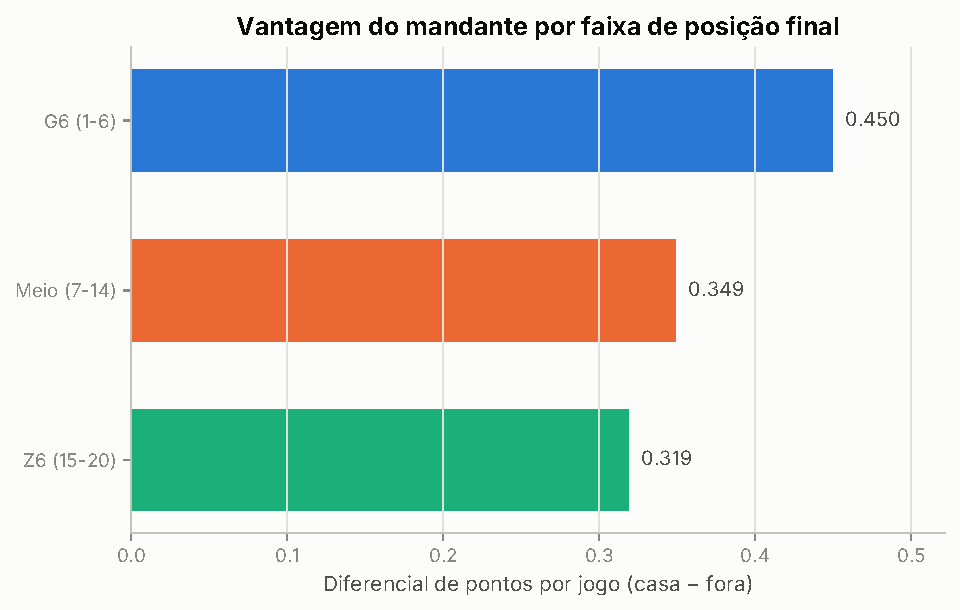
\includegraphics[width=0.75\textwidth]{./figuras/fator_casa_por_faixa.pdf}
  \fonte{Autoria própria (2026)}
\end{figure}

O resultado contraria a hipótese intuitiva. O gradiente é monotônico e aponta na
direção oposta: equipes que terminam entre as seis primeiras colocadas obtêm
vantagem de 0,450 ponto por partida ao jogar em casa, contra 0,349 das equipes
intermediárias e 0,319 das seis últimas. O mesmo ordenamento aparece em gols,
finalizações no alvo e escanteios, o que reduz a possibilidade de o achado ser
artefato de uma métrica específica.

A interpretação desse resultado deve considerar um efeito de teto. As equipes do
grupo G6 já conquistam, em média, 1,730 ponto por partida como visitantes,
restando-lhes apenas 1,270 ponto de margem até o máximo de três. As equipes do
Z6 conquistam 0,719 ponto fora e dispõem de 2,281 pontos de margem. Dispondo de
menos espaço para crescer, as equipes de maior qualidade ainda assim crescem
mais ao atuar em seus domínios. Normalizando o ganho pela margem disponível,
conforme a coluna de ganho relativo da Tabela~\ref{tab:clubes}, a diferença
entre os grupos torna-se ainda mais acentuada.

Esse achado tem implicação direta sobre a forma de operacionalizar o conceito de
qualidade técnica. A etapa anterior desta pesquisa comparava um grupo fixo de
seis clubes, convencionalmente denominado \textit{Big Six}, com os demais. Essa
operacionalização é problemática por duas razões: o grupo não é homogêneo ao
longo de um recorte de onze temporadas, e a comparação entre apenas dois grupos
descarta a informação ordinal da classificação. Quando a comparação é refeita
pela média do diferencial por clube, o grupo fixo apresenta 0,418 ponto contra
0,366 dos demais, diferença não significativa (Tabela~\ref{tab:testes},
$p = 0{,}351$), com intervalo de confiança compatível tanto com vantagem quanto
com desvantagem. A segmentação por posição final, por acompanhar a variação de
desempenho ao longo do tempo, revela a estrutura que a segmentação fixa não
captura.

\subsection{Variação entre Clubes}\label{sec:res-clubes}

A Tabela~\ref{tab:clubes} apresenta os clubes com maior diferencial no recorte,
restrita àqueles com pelo menos três temporadas disputadas.

\begin{table}[htb]
  \centering
  \caption{Clubes com maior diferencial casa--fora (mínimo de três temporadas).}
  \label{tab:clubes}
  \resizebox{\textwidth}{!}{% Gerado por scripts/gerar_tabelas_latex.py --- não editar à mão.
\begin{tabular}{lrrcrrrr}
  \toprule
  Clube & Jogos casa & Temp. & \textit{Big Six} & Pts casa & Pts fora & $\Delta$ pts & Ganho rel. \\
  \midrule
  Swansea & 57 & 3 & Não & 1,368 & 0,754 & +0,614 & 0,273 \\
  Arsenal & 209 & 11 & Sim & 2,201 & 1,612 & +0,589 & 0,424 \\
  Newcastle & 190 & 10 & Não & 1,626 & 1,058 & +0,568 & 0,293 \\
  Liverpool & 209 & 11 & Sim & 2,297 & 1,823 & +0,474 & 0,402 \\
  Sheffield United & 57 & 3 & Não & 1,035 & 0,596 & +0,439 & 0,182 \\
  Sunderland & 57 & 3 & Não & 1,246 & 0,807 & +0,439 & 0,200 \\
  Aston Villa & 152 & 8 & Não & 1,572 & 1,138 & +0,434 & 0,233 \\
  Man United & 209 & 11 & Sim & 1,952 & 1,531 & +0,421 & 0,287 \\
  Tottenham & 209 & 11 & Sim & 1,885 & 1,469 & +0,416 & 0,272 \\
  Brentford & 95 & 5 & Não & 1,537 & 1,126 & +0,411 & 0,219 \\
  \bottomrule
\end{tabular}
}
  \fonte{Autoria própria (2026)}
\end{table}

A restrição de amostra é necessária. Clubes que disputaram uma única temporada
no recorte acumulam apenas 19 partidas como mandantes, contra 209 dos clubes
presentes em todas as temporadas, e ocupam posições extremas do ranqueamento por
efeito da variabilidade amostral, e não por característica real de desempenho.

Entre os clubes com amostra suficiente, o diferencial varia de 0,614 ponto por
partida, no extremo superior, a 0,120 no inferior. A Figura~\ref{fig:dispersao}
posiciona cada clube segundo seu desempenho nas duas condições de mando: a
quase totalidade situa-se acima da linha de identidade, o que confirma que o
fenômeno afeta praticamente todos os competidores, ainda que em intensidades
distintas.

\begin{figure}[htb]
  \centering
  \caption{Desempenho das equipes como mandantes e como visitantes.}
  \label{fig:dispersao}
  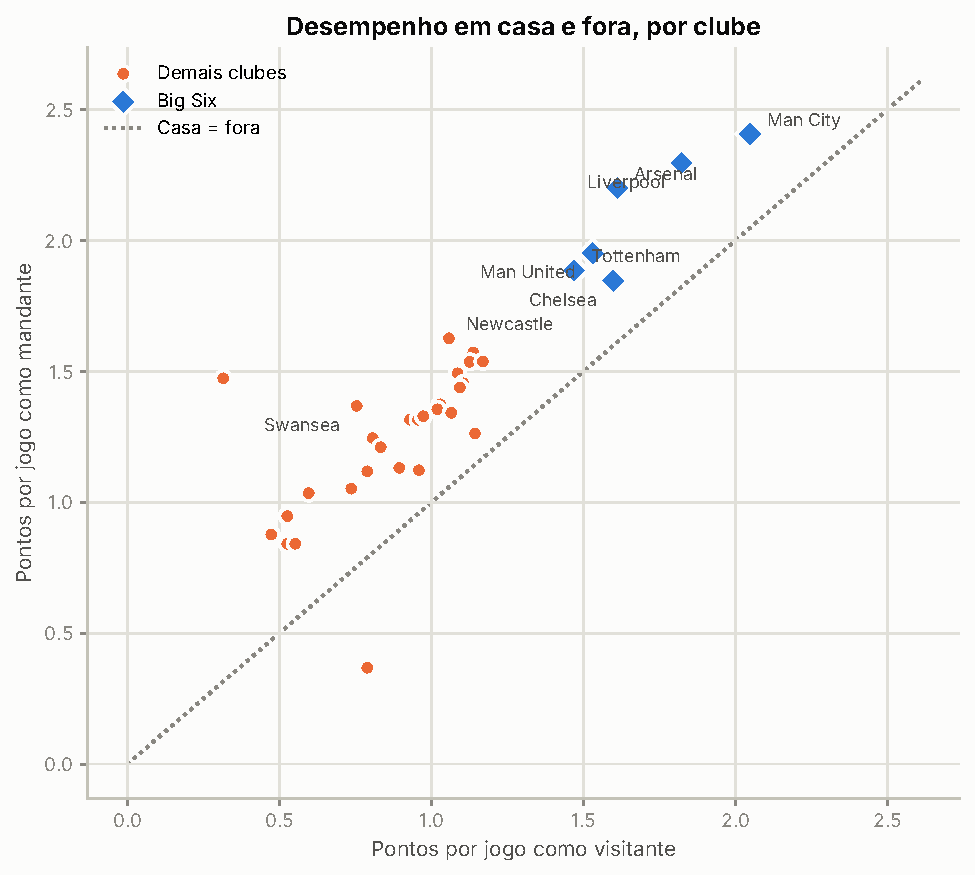
\includegraphics[width=0.72\textwidth]{./figuras/dispersao_casa_fora.pdf}
  \fonte{Autoria própria (2026)}
\end{figure}

\section{Evolução Temporal}\label{sec:res-temporal}

A Tabela~\ref{tab:evolucao} apresenta a evolução do diferencial de desempenho ao
longo das onze temporadas, incluindo métricas de volume ofensivo e disciplinares.

\begin{table}[htb]
  \centering
  \caption{Evolução temporal do diferencial entre mandantes e visitantes.}
  \label{tab:evolucao}
  \small
  % Gerado por scripts/gerar_tabelas_latex.py --- não editar à mão.
\begin{tabular}{lrrrrr}
  \toprule
  Temporada & $\Delta$ pts & Média móvel (3) & $\Delta$ chutes alvo & $\Delta$ escant. & $\Delta$ amarelos \\
  \midrule
  15/16 & +0,324 & --- & +0,747 & +1,061 & $-$0,208 \\
  16/17 & +0,616 & --- & +0,958 & +0,945 & $-$0,142 \\
  17/18 & +0,513 & +0,484 & +0,863 & +1,197 & $-$0,087 \\
  18/19 & +0,418 & +0,516 & +0,850 & +1,153 & $-$0,158 \\
  19/20 & +0,442 & +0,458 & +0,561 & +0,842 & $-$0,179 \\
  20/21 & $-$0,071 & +0,263 & +0,461 & +0,926 & $-$0,024 \\
  21/22 & +0,268 & +0,213 & +0,537 & +0,782 & $-$0,092 \\
  22/23 & +0,592 & +0,263 & +1,013 & +1,166 & $-$0,245 \\
  23/24 & +0,411 & +0,424 & +1,005 & +1,411 & $-$0,353 \\
  24/25 & +0,182 & +0,395 & +0,568 & +0,555 & $-$0,239 \\
  25/26 & +0,379 & +0,324 & +0,632 & +0,792 & $-$0,416 \\
  \bottomrule
\end{tabular}

  \fonte{Autoria própria (2026)}
\end{table}

O diferencial em pontos oscila de forma expressiva entre temporadas, de um
mínimo de $-0{,}071$ em 2020/21 a um máximo de $+0{,}616$ em 2016/17. A média
móvel de três temporadas situa-se entre 0,32 e 0,42 nas temporadas mais
recentes, contra valores entre 0,46 e 0,52 no início do período, padrão
compatível com uma redução moderada. As Figuras~\ref{fig:evolucao}
e~\ref{fig:diferencial} apresentam, respectivamente, as séries de pontos de
mandantes e visitantes e o diferencial entre elas.

\begin{figure}[htb]
  \centering
  \caption{Média de pontos por jogo de mandantes e visitantes, por temporada.}
  \label{fig:evolucao}
  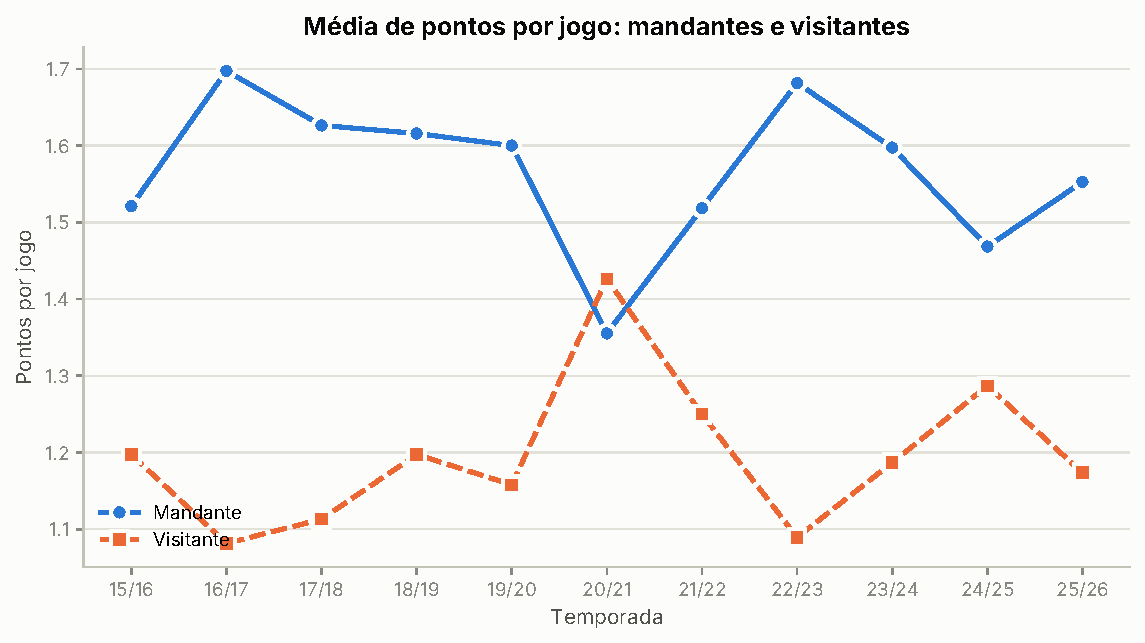
\includegraphics[width=0.9\textwidth]{./figuras/evolucao_pontos.pdf}
  \fonte{Autoria própria (2026)}
\end{figure}

\begin{figure}[htb]
  \centering
  \caption{Diferencial de pontos por jogo entre mandante e visitante.}
  \label{fig:diferencial}
  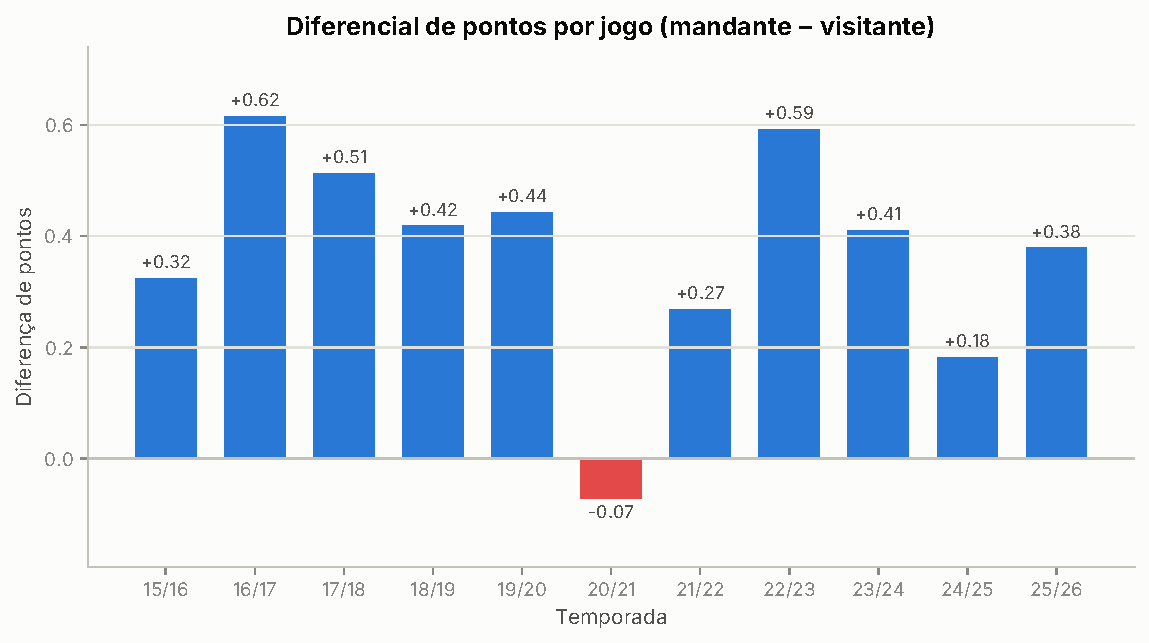
\includegraphics[width=0.9\textwidth]{./figuras/diferencial_por_temporada.pdf}
  \fonte{Autoria própria (2026)}
\end{figure}

As métricas de volume ofensivo acompanham o diferencial de pontos ao longo de
todo o período: os mandantes produzem, conforme a temporada, entre 0,46 e 1,01
finalização no alvo a mais e entre 0,56 e 1,41 escanteio a mais por partida. A
Figura~\ref{fig:volume} apresenta essa evolução.

\begin{figure}[htb]
  \centering
  \caption{Evolução das finalizações no alvo e dos escanteios por mando.}
  \label{fig:volume}
  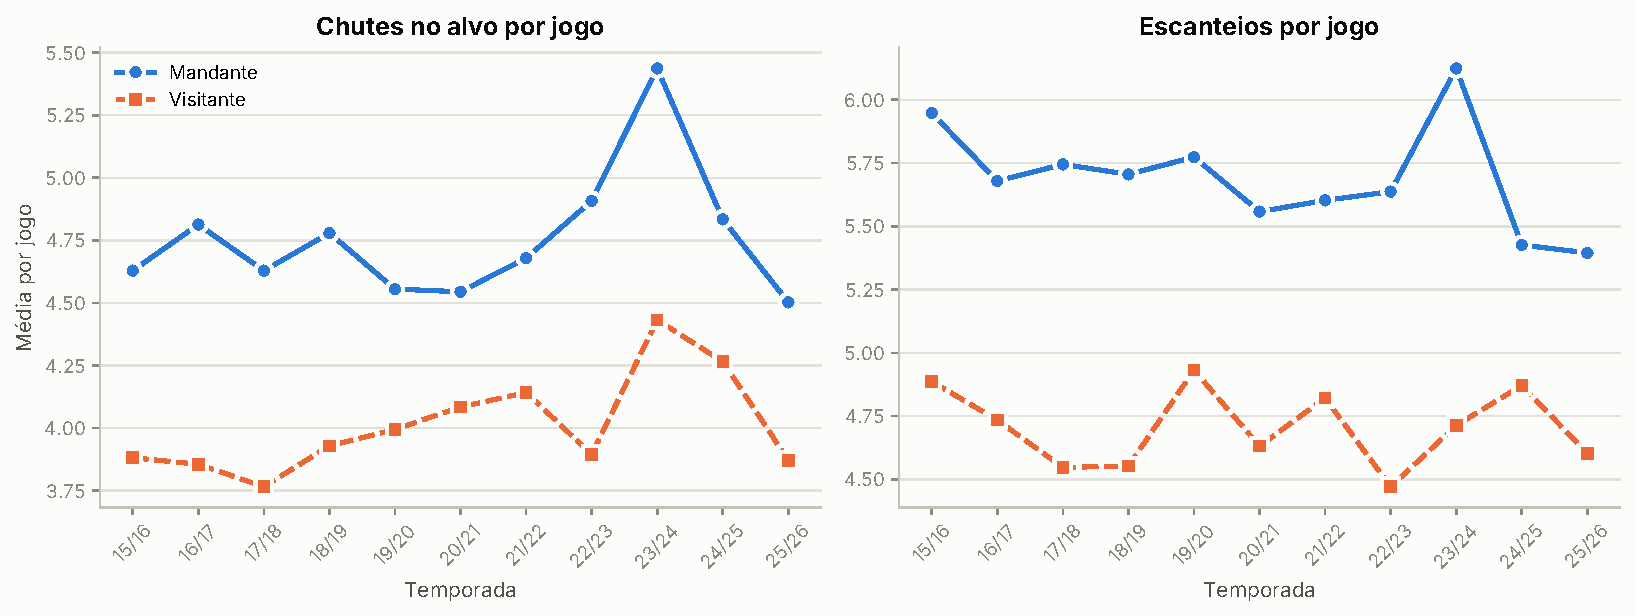
\includegraphics[width=\textwidth]{./figuras/volume_ofensivo.pdf}
  \fonte{Autoria própria (2026)}
\end{figure}

A coluna de cartões amarelos merece destaque. Em todas as temporadas o mandante
recebe menos cartões que o visitante, com diferencial que varia entre $-0{,}02$
e $-0{,}42$. A exceção é justamente 2020/21, temporada em que o diferencial
aproxima-se de zero ($-0{,}024$). Esse comportamento é retomado na
Seção~\ref{sec:res-publico}.

Cabe uma ressalva metodológica quanto à leitura de tendência. O diferencial bruto
de pontos de uma temporada depende não apenas da magnitude do Fator Casa, mas
também da distribuição de força entre os elencos daquele ano e do calendário
efetivamente sorteado. A Seção~\ref{sec:res-modelo} retoma essa questão com uma
métrica que controla por esses fatores.

\section{O Papel do Público}\label{sec:res-publico}

A literatura trata o período de portões fechados como um experimento natural
sobre o papel da torcida. A Tabela~\ref{tab:publico} apresenta o diferencial de
desempenho segundo o regime de público, classificado por data da partida
conforme descrito na Seção~\ref{sec:regime-publico}.

\begin{table}[htb]
  \centering
  \caption{Vantagem do mandante por regime de público.}
  \label{tab:publico}
  \resizebox{\textwidth}{!}{% Gerado por scripts/gerar_tabelas_latex.py --- não editar à mão.
\begin{tabular}{lrrrrrr}
  \toprule
  Cenário & Jogos & Pts casa & Pts fora & $\Delta$ pts & $\Delta$ gols & $\Delta$ amarelos \\
  \midrule
  2019/20 (sem público) & 92 & 1,620 & 1,163 & +0,457 & +0,370 & +0,033 \\
  2019/20 (com público) & 288 & 1,594 & 1,156 & +0,438 & +0,292 & $-$0,247 \\
  demais temporadas (com público) & 3420 & 1,587 & 1,175 & +0,411 & +0,302 & $-$0,215 \\
  2020/21 (público limitado) & 53 & 1,509 & 1,283 & +0,226 & +0,132 & $-$0,377 \\
  2020/21 (sem público) & 327 & 1,330 & 1,450 & $-$0,119 & $-$0,009 & +0,034 \\
  \bottomrule
\end{tabular}
}
  \fonte{Autoria própria (2026)}
\end{table}

\begin{figure}[htb]
  \centering
  \caption{Vantagem do mandante por regime de público.}
  \label{fig:publico}
  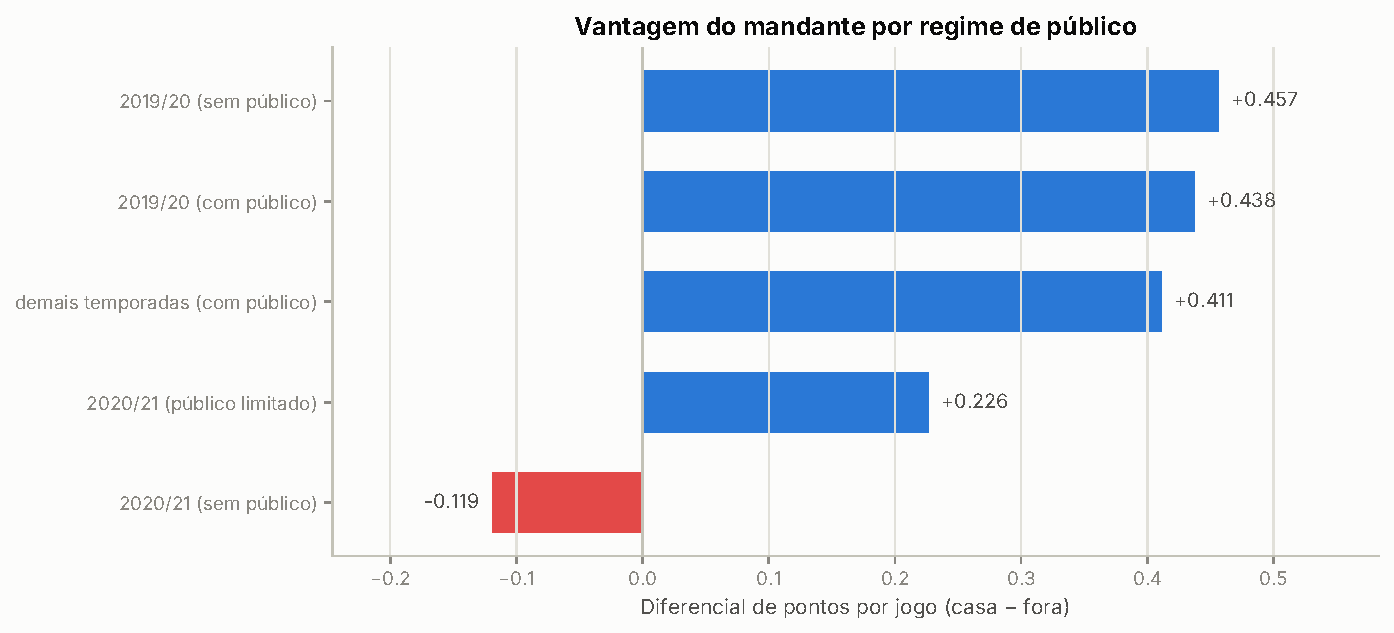
\includegraphics[width=0.95\textwidth]{./figuras/contraste_publico.pdf}
  \fonte{Autoria própria (2026)}
\end{figure}

O contraste decisivo encontra-se nas duas primeiras linhas da tabela. Dentro da
temporada 2019/20 — mesmos elencos, mesmo calendário e mesmo regulamento — as
92 partidas disputadas sem público apresentaram diferencial de $+0{,}457$ ponto,
contra $+0{,}438$ nas 288 partidas com público. A vantagem do mandante não
diminuiu com a ausência de torcida; se algo, foi marginalmente superior. A
diferença não é estatisticamente significativa (Tabela~\ref{tab:testes},
$p = 0{,}952$).

A inversão do Fator Casa manifesta-se exclusivamente em 2020/21, temporada na
qual o diferencial atinge $-0{,}119$ ponto. Essa constatação é relevante porque
2020/21 diferiu das temporadas anteriores em mais aspectos do que a ausência de
público: houve encurtamento da pré-temporada, congestionamento de calendário e
ampliação do número de substituições permitidas. Atribuir a queda
especificamente à ausência de torcida requer supor que nenhum desses fatores
contribuiu, suposição que o contraste de 2019/20 não corrobora.

\subsection{A Separação entre os Mecanismos}\label{sec:res-arbitragem}

A coluna de cartões amarelos da Tabela~\ref{tab:publico} permite uma distinção
que o diferencial de pontos, isoladamente, não permitiria.

Nas partidas com público, o mandante recebe sistematicamente menos cartões
amarelos que o visitante: $-0{,}247$ em 2019/20 e $-0{,}215$ nas demais
temporadas. Nas partidas sem público, essa vantagem desaparece, assumindo
valores praticamente nulos: $+0{,}033$ em 2019/20 e $+0{,}034$ em 2020/21.

O aspecto decisivo é que o desaparecimento ocorre \textbf{já em 2019/20}, mesma
temporada em que a vantagem em pontos não se alterou. Os dois fenômenos, portanto,
dissociam-se: a presença de torcida parece influenciar o comportamento da
arbitragem, conforme sugerido por~\citeonline{Nevill1999}, mas esse viés não é o
mecanismo que sustenta a vantagem do mandante em pontos. Trata-se de evidência a
favor da hipótese de que a familiaridade com o ambiente e o desgaste logístico
imposto ao visitante respondem por parcela mais relevante do fenômeno do que a
pressão da torcida sobre a arbitragem.

\section{Modelagem do Mando de Campo}\label{sec:res-modelo}

As seções anteriores apoiaram-se em médias condicionais, que não controlam pela
identidade dos adversários enfrentados. Esta seção apresenta os resultados do
modelo de Poisson bivariado descrito na Seção~\ref{sec:met-dixon-coles}.

Ajustado sobre o conjunto completo, o modelo estima um parâmetro de mando de
$\gamma = 0{,}1967$, com intervalo de confiança de 95\% entre 0,1605 e 0,2329.
Em termos interpretáveis, jogar em casa está associado a um acréscimo de
\textbf{21,7\% no número esperado de gols}, já descontada a qualidade do
adversário. O parâmetro de correção estimado é $\rho = -0{,}0388$, negativo
conforme previsto por~\citeonline{DixonColes1997}: o modelo de Poisson
independente subestima a frequência de empates de placar baixo.

As forças estimadas ordenam os clubes de maneira compatível com o desempenho
observado no período, com Manchester City e Liverpool no topo, o que constitui
verificação de consistência do ajuste.

\subsection{Evolução do Parâmetro de Mando}\label{sec:res-gamma-temporal}

A Tabela~\ref{tab:gamma} apresenta o parâmetro ajustado separadamente em cada
temporada, com os respectivos intervalos de confiança.

\begin{table}[htb]
  \centering
  \caption{Parâmetro de mando de campo ajustado, por temporada.}
  \label{tab:gamma}
  \small
  % Gerado por scripts/gerar_tabelas_latex.py --- não editar à mão.
\begin{tabular}{lrcr}
  \toprule
  Temporada & $\gamma$ & IC 95\% & Acréscimo de gols \\
  \midrule
  15/16 & 0,2107 & [0,088; 0,333] & 23,5\% \\
  16/17 & 0,2860 & [0,165; 0,407] & 33,1\% \\
  17/18 & 0,2944 & [0,171; 0,418] & 34,2\% \\
  18/19 & 0,2246 & [0,104; 0,345] & 25,2\% \\
  19/20 & 0,2311 & [0,109; 0,354] & 26,0\% \\
  20/21 & 0,0071 & [$-$0,115; 0,129] & 0,7\% \\
  21/22 & 0,1479 & [0,028; 0,268] & 15,9\% \\
  22/23 & 0,2913 & [0,171; 0,412] & 33,8\% \\
  23/24 & 0,1967 & [0,085; 0,308] & 21,7\% \\
  24/25 & 0,0627 & [$-$0,055; 0,180] & 6,5\% \\
  25/26 & 0,2145 & [0,093; 0,336] & 23,9\% \\
  \bottomrule
\end{tabular}

  \fonte{Autoria própria (2026)}
\end{table}

\begin{figure}[htb]
  \centering
  \caption{Parâmetro de mando ajustado por força do adversário, com IC de 95\%.}
  \label{fig:gamma}
  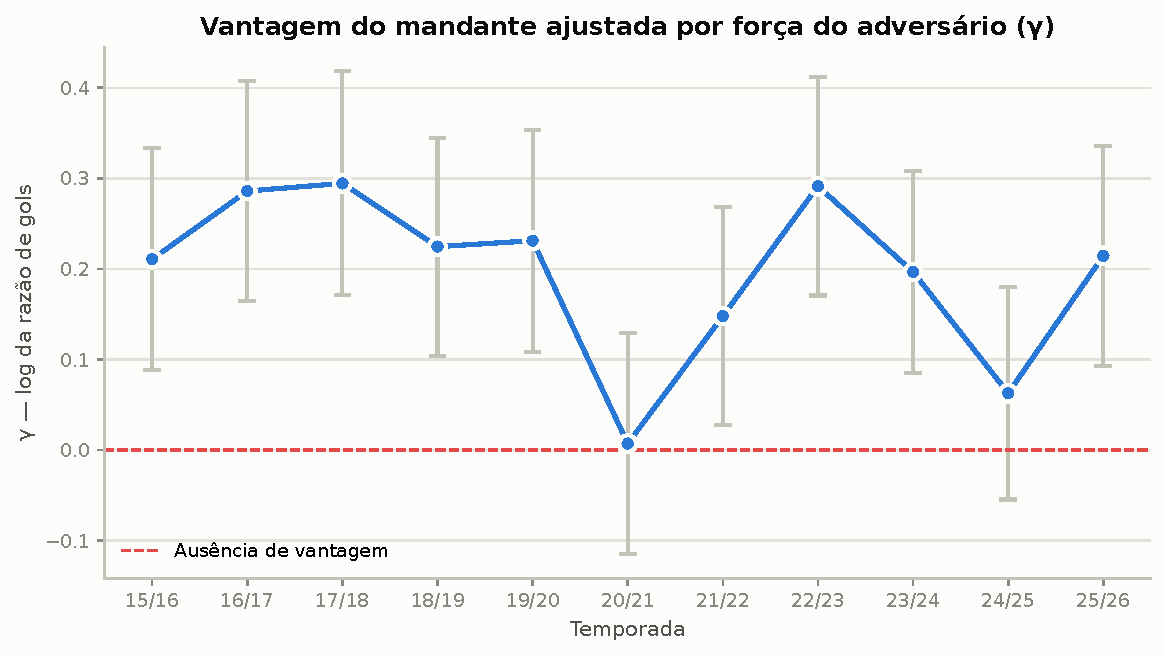
\includegraphics[width=0.95\textwidth]{./figuras/mando_ajustado_por_temporada.pdf}
  \fonte{Autoria própria (2026)}
\end{figure}

Duas temporadas apresentam intervalo de confiança que contém o zero, isto é,
nas quais não se pode rejeitar a hipótese de ausência de vantagem do mandante:
2020/21, já discutida, e \textbf{2024/25}, com $\gamma = 0{,}0627$ e intervalo
entre $-0{,}0547$ e $0{,}1801$. O segundo caso não guarda relação com a pandemia
e não se destacava com a mesma nitidez no diferencial bruto de pontos.

A disponibilidade dos intervalos de confiança impõe cautela à leitura de
tendência. Os intervalos de quase todas as temporadas se sobrepõem, e a
temporada 2022/23 ($\gamma = 0{,}2913$) situa-se no mesmo patamar de 2016/17 e
2017/18. O padrão compatível com os dados é o de \textbf{variabilidade elevada em
torno de um patamar estável, com dois vales}, e não o de uma tendência
monotônica de queda.

\subsection{Efeito do Público Controlado por Adversário}\label{sec:res-gamma-publico}

O contraste descritivo da Seção~\ref{sec:res-publico} não controla pela força
das equipes envolvidas, o que importa porque as partidas sem público de 2019/20
correspondem às rodadas finais, com distribuição de confrontos distinta da
temporada completa. A Tabela~\ref{tab:delta} apresenta a estimativa do
deslocamento~$\delta$ do parâmetro de mando associado à ausência de público.

\begin{table}[htb]
  \centering
  \caption{Efeito da ausência de público sobre o parâmetro de mando.}
  \label{tab:delta}
  \resizebox{\textwidth}{!}{% Gerado por scripts/gerar_tabelas_latex.py --- não editar à mão.
\begin{tabular}{lrrccr}
  \toprule
  Recorte & $\gamma$ & $\delta$ & IC 95\% & $p$ & $n$ sem / com \\
  \midrule
  2019/20 (intratemporada) & 0,2213 & +0,0402 & [$-$0,150; 0,231] & 0,680 & 92 / 288 \\
  recorte completo (19/20 + 20/21) & 0,2094 & $-$0,1225 & [$-$0,209; $-$0,036] & 0,006 & 419 / 3708 \\
  \bottomrule
\end{tabular}
}
  \fonte{Autoria própria (2026)}
\end{table}

Dentro da temporada 2019/20, a estimativa é $\delta = +0{,}0402$, com intervalo
entre $-0{,}1505$ e $+0{,}2308$ e $p = 0{,}680$: não há efeito detectável.
Considerando o conjunto das partidas sem público, a estimativa torna-se
$\delta = -0{,}1225$, com intervalo entre $-0{,}2095$ e $-0{,}0355$ e
$p = 0{,}006$, portanto significativa.

A conciliação entre os dois resultados é direta: 327 das 419 partidas sem
público pertencem à temporada 2020/21. O efeito agregado é determinado por essa
temporada. Convém explicitar o alcance dessa conclusão: o intervalo obtido para
2019/20 ainda contém o valor estimado no agregado, de modo que os dados
\textbf{não excluem} um efeito daquela magnitude. Tampouco é possível construir
o contraste dentro de 2020/21, pois nenhuma partida daquela temporada foi
disputada com público pleno segundo a classificação adotada.

O que se pode afirmar com segurança é que a vantagem do mandante reduziu-se
praticamente a zero em 2020/21, e que a atribuição dessa redução especificamente
à ausência de torcida é uma inferência que o contraste intratemporada disponível
não corrobora. Essa conclusão diverge de parte da literatura que tratou o
episódio como isolamento limpo da variável público e, à luz da dissociação
apresentada na Seção~\ref{sec:res-arbitragem}, sugere que o papel da torcida
opera preferencialmente sobre o comportamento da arbitragem.

\section{Modelagem Preditiva}\label{sec:res-preditivo}

A Tabela~\ref{tab:preditivo} apresenta o desempenho dos modelos preditivos sob
validação temporal, agregado sobre as oito temporadas de teste, totalizando
3.040 partidas.

\begin{table}[htb]
  \centering
  \caption{Desempenho preditivo sob validação temporal.}
  \label{tab:preditivo}
  \small
  % Gerado por scripts/gerar_tabelas_latex.py --- não editar à mão.
\begin{tabular}{lrrrr}
  \toprule
  Modelo & \textit{Log-loss} & Brier & Acurácia & $n$ \\
  \midrule
  Dixon-Coles & 0,9762 & 0,5785 & 53,6\% & 3040 \\
  Regressão logística & 0,9880 & 0,5834 & 53,6\% & 3040 \\
  Frequência base & 1,0669 & 0,6457 & 43,9\% & 3040 \\
  Sempre o mandante & 1,0747 & 0,6500 & 43,9\% & 3040 \\
  \textit{Gradient boosting} & 1,0807 & 0,6257 & 50,7\% & 3040 \\
  \bottomrule
\end{tabular}

  \fonte{Autoria própria (2026)}
\end{table}

\begin{figure}[htb]
  \centering
  \caption{Desempenho preditivo dos modelos avaliados.}
  \label{fig:preditivo}
  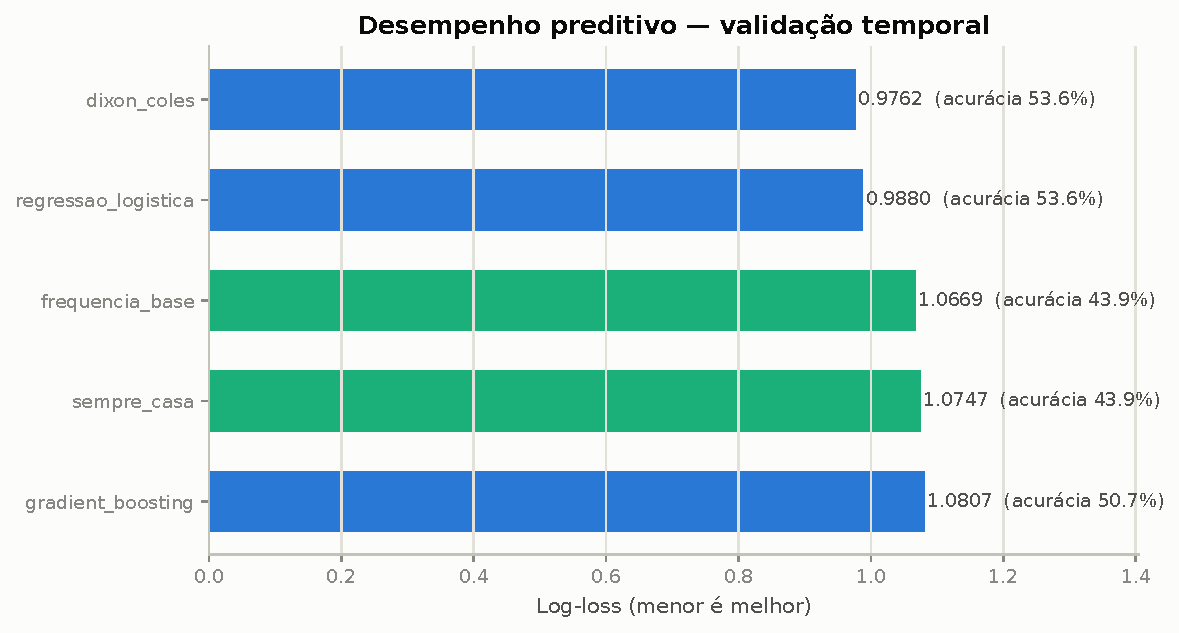
\includegraphics[width=0.9\textwidth]{./figuras/preditivo_desempenho.pdf}
  \fonte{Autoria própria (2026)}
\end{figure}

Três leituras merecem destaque.

A primeira é que \textbf{o modelo estatístico superou os modelos de aprendizado
de máquina}. O modelo de Poisson bivariado obteve o menor \textit{log-loss}
(0,9762) e o menor escore de Brier (0,5785), liderando em seis das oito
temporadas avaliadas, com a regressão logística em posição próxima (0,9880).
Esse resultado é coerente com a natureza do problema: o modelo de Poisson
incorpora a estrutura geradora dos dados — gols são contagens, cada clube possui
capacidades distintas de ataque e defesa, e o mando desloca a média esperada —
em vez de precisar inferi-la a partir de um conjunto limitado de variáveis
explicativas.

A segunda é que \textbf{o modelo de \textit{gradient boosting} obteve desempenho
inferior ao da frequência base} segundo o \textit{log-loss} (1,0807 contra
1,0669), apesar de apresentar acurácia substancialmente superior (50,66\% contra
43,95\%). Essa combinação é característica de um modelo mal calibrado e
constitui a justificativa empírica para a escolha de métricas discutida na
Seção~\ref{sec:avaliacao}.

A terceira é que todos os modelos superam a heurística de prever sempre a
vitória do mandante, que atinge 43,95\% de acurácia, contra 53,59\% do modelo de
Poisson. O ganho é real, porém modesto, o que evidencia o teto de
previsibilidade característico da modalidade.

\subsection{Análise de Calibração}\label{sec:res-calibracao}

A Figura~\ref{fig:calibracao} compara, em faixas de probabilidade prevista, a
frequência efetivamente observada de vitórias do mandante.

\begin{figure}[htb]
  \centering
  \caption{Curvas de calibração para a previsão de vitória do mandante.}
  \label{fig:calibracao}
  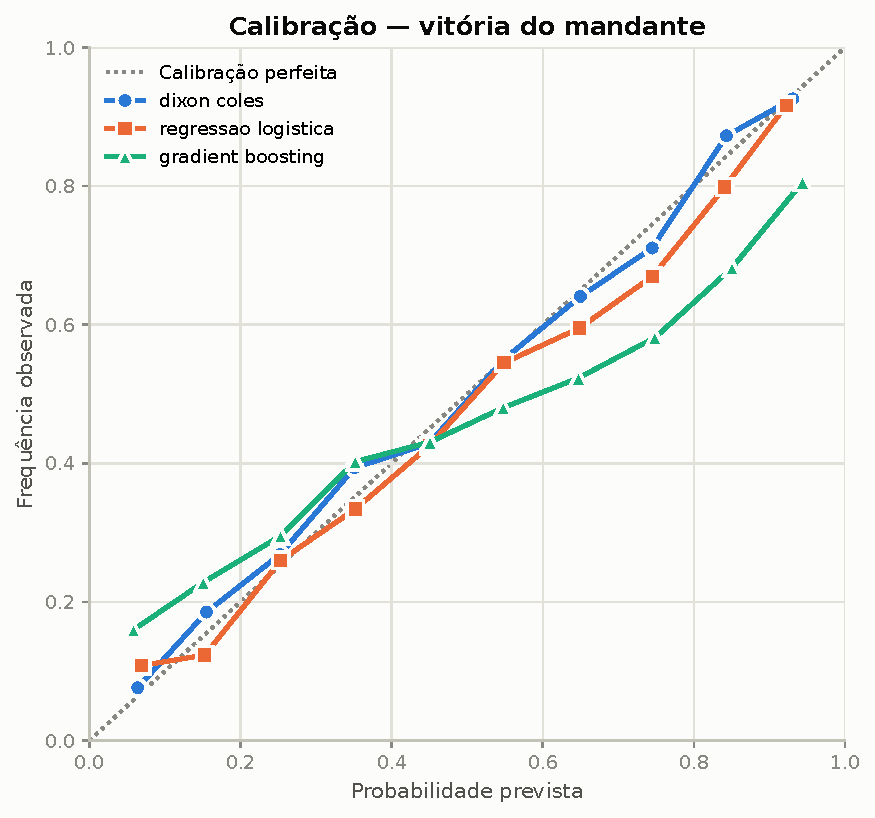
\includegraphics[width=0.72\textwidth]{./figuras/preditivo_calibracao.pdf}
  \fonte{Autoria própria (2026)}
\end{figure}

O modelo de Poisson e a regressão logística situam-se próximos à diagonal, o que
indica boa calibração. O modelo de \textit{gradient boosting}, por sua vez,
apresenta desvio sistemático em ambos os extremos: nas partidas às quais atribui
94\% de probabilidade de vitória do mandante, a frequência observada é de 81\%;
naquelas às quais atribui 6\%, o evento ocorre em 16\% dos casos.

O comportamento é internamente consistente com as métricas da
Tabela~\ref{tab:preditivo}. Ao deslocar as probabilidades em direção aos
extremos, o modelo acerta mais frequentemente a classe mais provável — o que
eleva a acurácia — e simultaneamente incorre em penalizações severas do
\textit{log-loss} nas previsões confiantes e incorretas. Esse resultado ilustra,
de forma concreta, por que a acurácia é insuficiente como critério único de
avaliação em problemas probabilísticos.

Observa-se ainda que todos os modelos apresentam desempenho pior na temporada
2020/21. Na ausência da vantagem do mandante, o preditor mais informativo do
problema perde força, e a previsão torna-se mais difícil para todos os métodos
avaliados — resultado que conecta a etapa preditiva à análise do Fator Casa
conduzida nas seções anteriores.

\section{Estudo de Caso: Mudança de Estádio}\label{sec:resultados-estadios}

A arquitetura e a atmosfera do estádio constituem variável qualitativa
frequentemente associada ao Fator Casa. Esta seção examina o desempenho de
clubes que mudaram de sede durante o período analisado.

A análise exige recorte estendido, iniciado em 2009/10, pois o recorte principal
não oferece linha de base anterior às mudanças. Conforme a
Seção~\ref{sec:quebras}, métricas de finalização não são comparáveis através da
fronteira de 2013/14 e, por essa razão, foram omitidas da
Tabela~\ref{tab:estadios}. O Brentford, que disputou a \textit{Premier League}
apenas a partir de 2021/22, já em sua nova sede, não possui período anterior e
foi excluído da análise.

\begin{table}[htb]
  \centering
  \caption{Desempenho antes e depois da mudança de estádio.}
  \label{tab:estadios}
  \resizebox{\textwidth}{!}{% Gerado por scripts/gerar_tabelas_latex.py --- não editar à mão.
\begin{tabular}{lllrrrr}
  \toprule
  Clube & Período & Estádio & Jogos casa & Pts casa & Pts fora & $\Delta$ pts \\
  \midrule
  West Ham & Antes & Boleyn Ground (Upton Park) & 114 & 1,474 & 0,826 & +0,648 \\
  West Ham & Depois & London Stadium & 190 & 1,421 & 1,074 & +0,347 \\
  Tottenham & Antes & White Hart Lane / Wembley & 185 & 2,103 & 1,654 & +0,448 \\
  Tottenham & Depois & Tottenham Hotspur Stadium & 138 & 1,696 & 1,281 & +0,414 \\
  \bottomrule
\end{tabular}
}
  \fonte{Autoria própria (2026)}
\end{table}

O West Ham United apresentou redução expressiva: de $+0{,}648$ ponto por partida
no Boleyn Ground para $+0{,}347$ no London Stadium, aproximadamente metade da
vantagem anterior. O Tottenham Hotspur, por sua vez, manteve desempenho
praticamente inalterado, passando de $+0{,}448$ para $+0{,}414$.

O resultado é sugestivo e compatível com a hipótese de que arenas modernas, de
maior capacidade e com afastamento entre arquibancada e campo, diluiriam a
pressão exercida sobre o visitante. Deve, contudo, ser interpretado como
\textbf{estudo de caso exploratório}. São apenas dois clubes, e os períodos
posteriores às mudanças coincidem com alterações de elenco, de comissão técnica e
de patamar competitivo que não foram controladas. A evidência é insuficiente para
sustentar afirmação causal.


%% Conclusão
%%%% CAPÍTULO 5 - CONCLUSÃO

\chapter{Conclusão}\label{cap:conclusao}

[Capítulo em elaboração.]

\section{Limitações}\label{sec:limitacoes}

[Seção em elaboração.]

\section{Trabalhos Futuros}\label{sec:trabalhos-futuros}

[Seção em elaboração.]


%% Parte
% \part{Conclusão}%% Comente para remover este item

%% Capítulo
%\include{./capitulos/cap-conclusoes}%% Comente para remover este item

%% Capítulos após este comando criam marcadores do pdf na raiz
% \phantompart%% Comente para remover este item


%% Formatação de páginas de elementos pós-textuais
\postextual%% Não comente esta linha

%% Arquivos de referências
\arquivosdereferencias{%% Arquivos bibtex sem a extensão .bib e separados por vírgula - Não comente esta linha
  %./PosTexto/exemplos-referencias,%% Arquivo de referências - Comente para remover este item
  main%% Arquivo de referências - Comente para remover este item
}%% Não comente esta linha

%% Glossário
%\incluirglossario %% Comente para remover este item

\renewcommand{\ABNTEXchapterfont}{\bfseries}
\renewcommand{\ABNTEXchapterfontsize}{\normalsize}
\renewcommand{\thechapter}{\Alph{chapter}} % Letra ao invés de número
\renewcommand{\chaptername}{Apêndice} % Muda a palavra "Capítulo" para "Apêndice"

%% Arquivos de apêndices
\begin{arquivosdeapendices}%% Os arquivos de apêndices devem se incluídos neste ambiente - Não comente esta linha
%  \partapendices%% Página de início dos apêndices - adiciona uma página com o título Apêndices
%   %% Capítulo de exemplo
%\begin{apendicesenv}
%   %%%% APÊNDICE A
    \cleardoublepage
    \thispagestyle{empty}
    \refstepcounter{chapter} % incrementa o contador
    %\chapter*{Apêndice~\thechapter\\[1ex]Questionário de pesquisa}   
    \vspace*{\fill}
    \begin{center}
        {\bfseries APÊNDICE~\thechapter{ -- }Questionário de pesquisa}
    \end{center}
    \vspace*{\fill}
    \addcontentsline{toc}{chapter}{APÊNDICE~\thechapter{ -- } Questionário de pesquisa}

%\chapter{Questionário de pesquisa}\label{cap:apendicea}
\newpage
\centerline{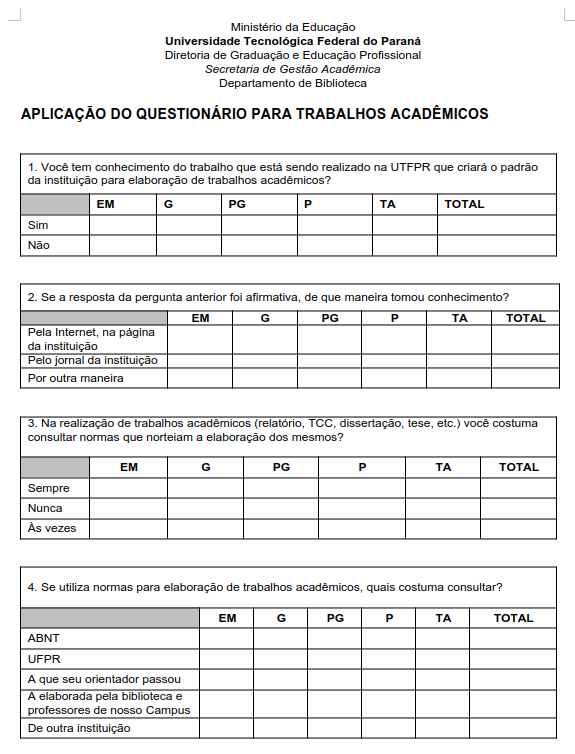
\includegraphics[width=\textwidth]{./PosTexto/Ilustracoes/questionario}}%% Imagem (Dimensões e localização)%% Apêndice - Comente para remover este item
%   
%\chapter{Roteiro da entrevista}\label{cap:apendiceb}
%\apendices

    \cleardoublepage
    \thispagestyle{empty}
    \refstepcounter{chapter} % incrementa o contador
    %\chapter*{Apêndice~\thechapter\\[1ex]Questionário de pesquisa}   
    \vspace*{\fill}
    \begin{center}
        {\bfseries APÊNDICE~\thechapter{ -- }Roteiro da entrevista}
    \end{center}
    \vspace*{\fill}
    \addcontentsline{toc}{chapter}{APÊNDICE~\thechapter{ -- } Roteiro da entrevista}

\newpage
\centerline{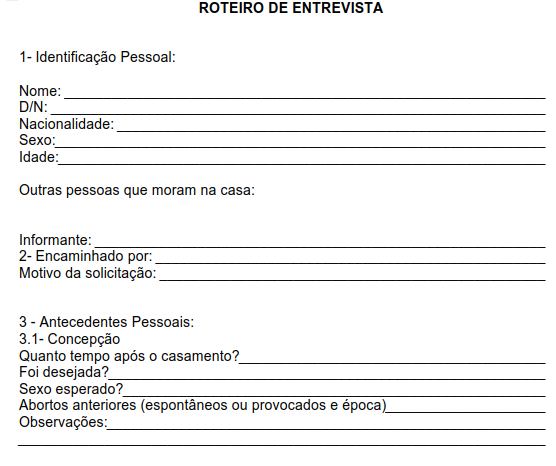
\includegraphics[width=\textwidth]{./PosTexto/Ilustracoes/roteiro}}%% Imagem (Dimensões e localização)%% Apêndice - Comente para remover este item
%   
    \cleardoublepage
    \thispagestyle{empty}
    \refstepcounter{chapter} % incrementa o contador
    %\chapter*{Apêndice~\thechapter\\[1ex]Questionário de pesquisa}   
    \vspace*{\fill}
    \begin{center}
        {\bfseries APÊNDICE~\thechapter{ -- }Abreviaturas dos meses do ano}
    \end{center}
    \vspace*{\fill}
    \addcontentsline{toc}{chapter}{APÊNDICE~\thechapter{ -- } Abreviaturas dos meses do ano}
    
%\chapter{Abreviaturas dos meses do ano}\label{cap:apendicec}
\newpage

%\centerline{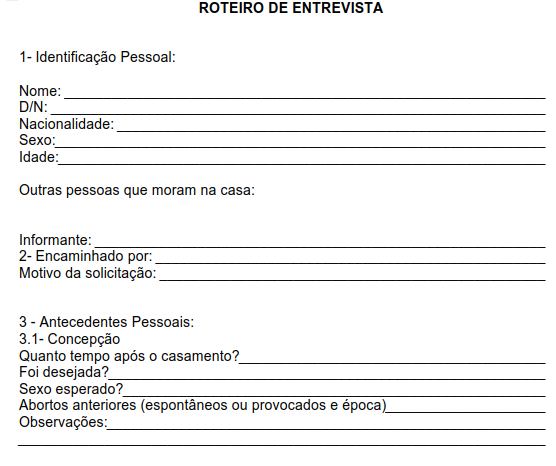
\includegraphics[width=\textwidth]{./PosTexto/Ilustracoes/roteiro}}%% Imagem (Dimensões e localização)

\begin{center}
\textbf{Abreviaturas dos meses do ano}    
\end{center}


\doublespacing{

\begin{tabular}{l l}
Janeiro –  &  jan. \\
Fevereiro –  & fev. \\
Março –  &mar.\\
Abril –   &abr.\\
Maio –  &maio (único não abreviado).\\
Junho –   &jun. \\
Julho –   &jul.\\
Agosto –  &ago.\\
Setembro –  &set.\\
Outubro –  &out.\\
Novembro –  &nov.\\
Dezembro –  &dez.\\
\end{tabular}
}%% Apêndice - Comente para remover este item
%\end{apendicesenv}
\end{arquivosdeapendices}%% Não comente esta linha


% \begin{apendicesenv}%% Ambiente apendicesenv

% %\partapendices
% % \chapter{Ola}

% % \lipsum[55-56]

% \end{apendicesenv}

%% Arquivos de anexos
\begin{arquivosdeanexos}%% Os arquivos de anexos devem se incluídos neste ambiente - Não comente esta linha
  %\partanexos%% Página de início dos anexos - adiciona uma página com o título Anexosm
%   %%%% ANEXO A
%%
%% Texto ou documento não elaborado pelo autor, que serve de fundamentação, comprovação e ilustração.

%% Título e rótulo de anexo (rótulos não devem conter caracteres especiais, acentuados ou cedilha)
\anexos
  \cleardoublepage
    \thispagestyle{empty}
    \refstepcounter{chapter} % incrementa o contador
    %\chapter*{Apêndice~\thechapter\\[1ex]Questionário de pesquisa}   
    \vspace*{\fill}
    \begin{center}
        {\bfseries ANEXO~\thechapter{ -- }Lei N\texorpdfstring{.\textsuperscript{o}}{o.} 9.610, de 19 de Fevereiro de 1998}
    \end{center}
    \vspace*{\fill}
    \addcontentsline{toc}{chapter}{ANEXO~\thechapter{ -- }Lei N\texorpdfstring{.\textsuperscript{o}}{o.} 9.610, de 19 de Fevereiro de 1998}

%\chapter{Lei N\texorpdfstring{.\textsuperscript{o}}{o.} 9.610, de 19 de Fevereiro de 1998}\label{cap:anexoa}


\newpage
\centerline{
\includegraphics[width=\textwidth]{./PosTexto/Ilustracoes/top.png}}%% Imagem (Dimensões e localização)

\begin{center}
\textbf{LEI Nº 9.610, DE 19 DE FEVEREIRO DE 1998\footnote{Disponível em:\url{http://www.planalto.gov.br/ccivil_03/leis/l9610.htm.}}.}
\end{center}

\hspace{7cm}\parbox{8cm}{\scriptsize{\textcolor{red}{Altera, atualiza e consolida a legislação sobre direitos autorais e dá outras providências.}}}
\vspace{0.3cm}

\textbf{O PRESIDENTE DA REPÚBLICA} Faço saber que o Congresso Nacional decreta e eu sanciono a seguinte Lei:

\begin{center}
Título I - Disposições Preliminares
\end{center}

\scriptsize{
Art. 1º Esta Lei regula os direitos autorais, entendendo-se sob esta denominação os direitos de autor e os que lhes são conexos. 

Art. 2º Os estrangeiros domiciliados no exterior gozarão da proteção assegurada nos acordos, convenções e tratados em vigor no Brasil.

Parágrafo único. Aplica-se o disposto nesta Lei aos nacionais ou pessoas domiciliadas em país que assegure aos brasileiros ou pessoas domiciliadas no Brasil a reciprocidade na proteção aos direitos autorais ou equivalentes.

Art. 3º Os direitos autorais reputam-se, para os efeitos legais, bens móveis.

Art. 4º Interpretam-se restritivamente os negócios jurídicos sobre os direitos autorais.

Art. 5º Para os efeitos desta Lei, considera-se:

I - publicação - o oferecimento de obra literária, artística ou científica ao conhecimento do público, com o consentimento do autor, ou de qualquer outro titular de direito de autor, por qualquer forma ou processo;

II - transmissão ou emissão - a difusão de sons ou de sons e imagens, por meio de ondas radioelétricas; sinais de satélite; fio, cabo ou outro condutor; meios óticos ou qualquer outro processo eletromagnético; 

III - retransmissão - a emissão simultânea da transmissão de uma empresa por outra;

IV - distribuição - a colocação à disposição do público do original ou cópia de obras literárias, artísticas ou científicas, interpretações ou execuções fixadas e fonogramas, mediante a venda, locação ou qualquer outra forma de transferência de propriedade ou posse;

V - comunicação ao público - ato mediante o qual a obra é colocada ao alcance do público, por qualquer meio ou procedimento e que não consista na distribuição de exemplares;

VI - reprodução - a cópia de um ou vários exemplares de uma obra literária, artística ou científica ou de um fonograma, de qualquer forma tangível, incluindo qualquer armazenamento permanente ou temporário por meios eletrônicos ou qualquer outro meio de fixação que venha a ser desenvolvido;

VII - contrafação - a reprodução não autorizada;

VIII - obra: 

a) em co-autoria - quando é criada em comum, por dois ou mais autores;

b) anônima - quando não se indica o nome do autor, por sua vontade ou por ser desconhecido;

c) pseudônima - quando o autor se oculta sob nome suposto;

d) inédita - a que não haja sido objeto de publicação;

e) póstuma - a que se publique após a morte do autor;

f) originária - a criação primígena;

g) derivada - a que, constituindo criação intelectual nova, resulta da transformação de obra originária;

h) coletiva - a criada por iniciativa, organização e responsabilidade de uma pessoa física ou jurídica, que a publica sob seu nome ou marca e que é constituída pela participação de diferentes autores, cujas contribuições se fundem numa criação autônoma;

i) audiovisual - a que resulta da fixação de imagens com ou sem som, que tenha a finalidade de criar, por meio de sua reprodução, a impressão de movimento, independentemente dos processos de sua captação, do suporte usado inicial ou posteriormente para fixá-lo, bem como dos meios utilizados para sua veiculação;

IX - fonograma - toda fixação de sons de uma execução ou interpretação ou de outros sons, ou de uma representação de sons que não seja uma fixação incluída em uma obra audiovisual;

X - editor - a pessoa física ou jurídica à qual se atribui o direito exclusivo de reprodução da obra e o dever de divulgá-la, nos limites previstos no contrato de edição; 

XI - produtor - a pessoa física ou jurídica que toma a iniciativa e tem a responsabilidade econômica da primeira fixação do fonograma ou da obra audiovisual, qualquer que seja a natureza do suporte utilizado;

XII - radiodifusão - a transmissão sem fio, inclusive por satélites, de sons ou imagens e sons ou das representações desses, para recepção ao público e a transmissão de sinais codificados, quando os meios de decodificação sejam oferecidos ao público pelo organismo de radiodifusão ou com seu consentimento;

XIII - artistas intérpretes ou executantes - todos os atores, cantores, músicos, bailarinos ou outras pessoas que representem um papel, cantem, recitem, declamem, interpretem ou executem em qualquer forma obras literárias ou artísticas ou expressões do folclore.

Art. 6º Não serão de domínio da União, dos Estados, do Distrito Federal ou dos Municípios as obras por eles simplesmente subvencionadas.
}

%% Anexo - Comente para remover este item
\end{arquivosdeanexos}%% Não comente esta linha

%% Índice - Adiciona um índice remissivo.
%\incluirindice%% Comente para remover este item

%% Fim do documento
\end{document}%% Não comente esta linha
